\section{Présentation}
\ifprof
\else
\subsection{Contexte}
L'utilisation du mode vidéo, en haute définition sur les appareils photo réflex et légers, pose aux photographes le problème de la stabilisation de l'image car les vibrations engendrées y sont importantes et visibles. Des stabilisateurs installés à l'intérieur des appareils diminuent l'effet de ces vibrations mais ils restent très insuffisants pour assurer une bonne stabilisation notamment sur des sujets mobiles car ces systèmes ne sont efficaces que pour des temps de pose relativement longs. C'est pour cette raison que des systèmes de stabilisation externes ont été développés avec des supports et accessoires purement mécaniques ou motorisés.

\subsection{Nacelles gyrostabilisées}
Parmi les systèmes de stabilisation externes, les nacelles gyrostabilisées, installées sur une perche portée par les deux mains de l'utilisateur et sur lesquelles se fixe l'appareil photographique présentent l'avantage d'être légères, compactes et d'utilisation facile. Elles permettent de corriger les perturbations dues aux mouvements de l'utilisateur selon trois axes de rotations (figure~\ref{fig:01}). Néanmoins, elles ne permettent pas de réduire les perturbations verticales dues à la marche ou à la course de l'utilisateur.

\begin{figure}[H]
\centering
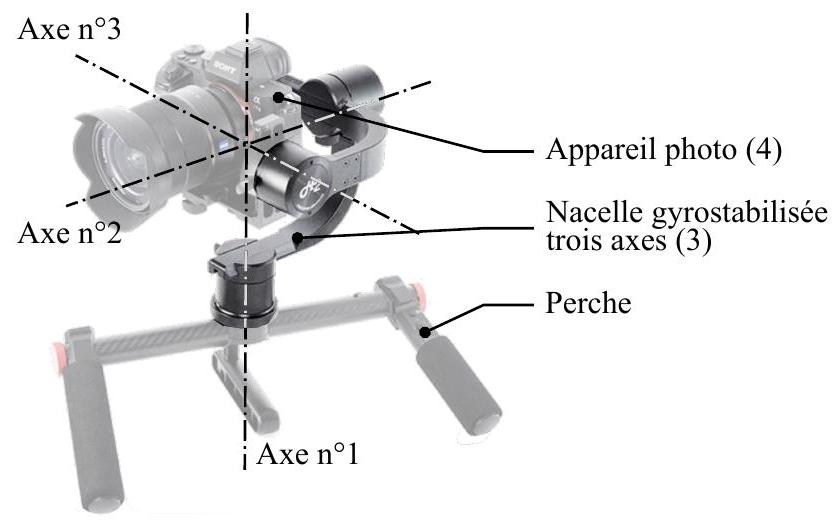
\includegraphics[width=.5\textwidth]{fig_01.jpg}
\caption{\label{fig:01} Nacelle gyrostabilisée}
\end{figure}


\subsection{Stabilisateur vertical}
Pour maitriser les perturbations verticales dues à la marche ou la course des photographes, un constructeur commercialise un stabilisateur vertical à installer entre la perche et la nacelle gyrostabilisée (figure~\ref{fig:02}).

\begin{figure}[H]
\centering
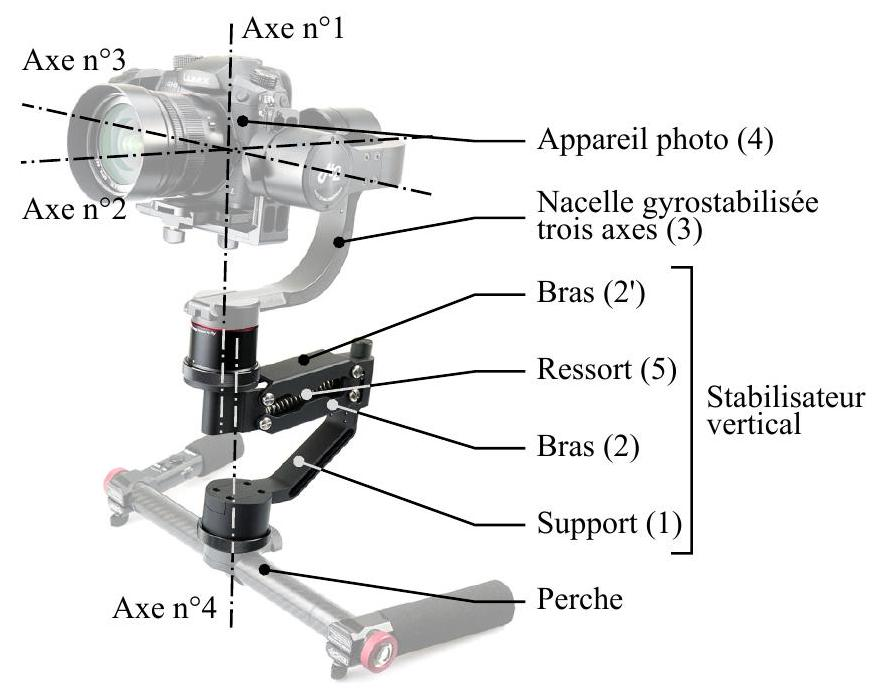
\includegraphics[width=.5\textwidth]{fig_02.jpg}
\caption{\label{fig:02} Nacelle gyrostabilisée avec stabilisateur vertical}
\end{figure}


Une analyse du besoin des photographes a permis de documenter le cahier des charges fonctionnel dont un extrait est donné figure~\ref{fig:A} du document réponse. Le cadre de ce sujet porte plus spécifiquement sur l'évaluation des solutions retenues pour satisfaire les objectifs de maitrise de la position d'un appareil photo à l'équilibre et en mouvement. Le sujet est décomposé en quatre parties :

\begin{itemize}
  \item dans la partie \ref{part:1}, une analyse des mouvements de marche et de course d'un utilisateur est effectuée et les critères chiffrés de l'exigence relative à la position de l'appareil photo en mouvement sont justifiés ;
  \item la partie \ref{part:2} porte sur la vérification du respect de l'exigence relative à la position à l'équilibre de l'appareil photo ;
  \item en partie \ref{part:3}, une étude dynamique met en évidence la nécessité d'ajouter une commande active au système pour assurer le respect de l'exigence relative à la position en mouvement de l'appareil photo ;
  \item la partie \ref{part:4} porte sur la conception de la commande active du système en vue d'assurer la maitrise de la position de l'appareil photo avec le niveau de précision requis par le cahier des charges.
\end{itemize}

\fi

\section{\label{part:1}Analyse du mouvement de l'utilisateur et justification du cahier des charges }

\ifprof
\else
\begin{obj}
Analyser les mouvements de l’utilisateur lorsqu’il marche ou lorsqu’il court et justifier les critères
chiffrés de l’exigence relative à la position de l’appareil photo en mouvement
\end{obj}



Pour réduire les perturbations verticales de l'appareil photo, la solution retenue est de filtrer les mouvements de translation verticale de la perche dont les fréquences sont précisées dans le cahier des charges (\ref{fig:A}). Pour justifier ces performances, on réalise des captures du mouvement vertical d'une perche tenue des deux mains par un utilisateur qui se déplace sur un sol plat.

Cette capture de mouvement est réalisée à partir d'un système optoélectronique dont le principe est le suivant : des caméras projettent une lumière dans le spectre infrarouge et détectent la lumière réfléchie par des marqueurs réfléchissants placés sur l'utilisateur. À partir des focales des caméras, de leur position et de leur orientation, il est possible de reconstruire, à chaque instant, par triangulation, la position spatiale des marqueurs et d'en déduire le mouvement vertical des mains, en retenant la valeur moyenne de la position verticale des deux mains. Les graphes des enregistrements de deux passages, marche et course, sont donnés ainsi que leur analyse spectrale (figure~\ref{fig:03}). Le contenu spectral est estimé en utilisant un enregistrement sur une durée limitée et la relation utilisée permet d'obtenir directement les amplitudes des différentes composantes harmoniques. Le calcul du spectre est réalisé pour un ensemble de fréquences choisi selon une distribution linéaire.


\begin{figure}[H]
\centering
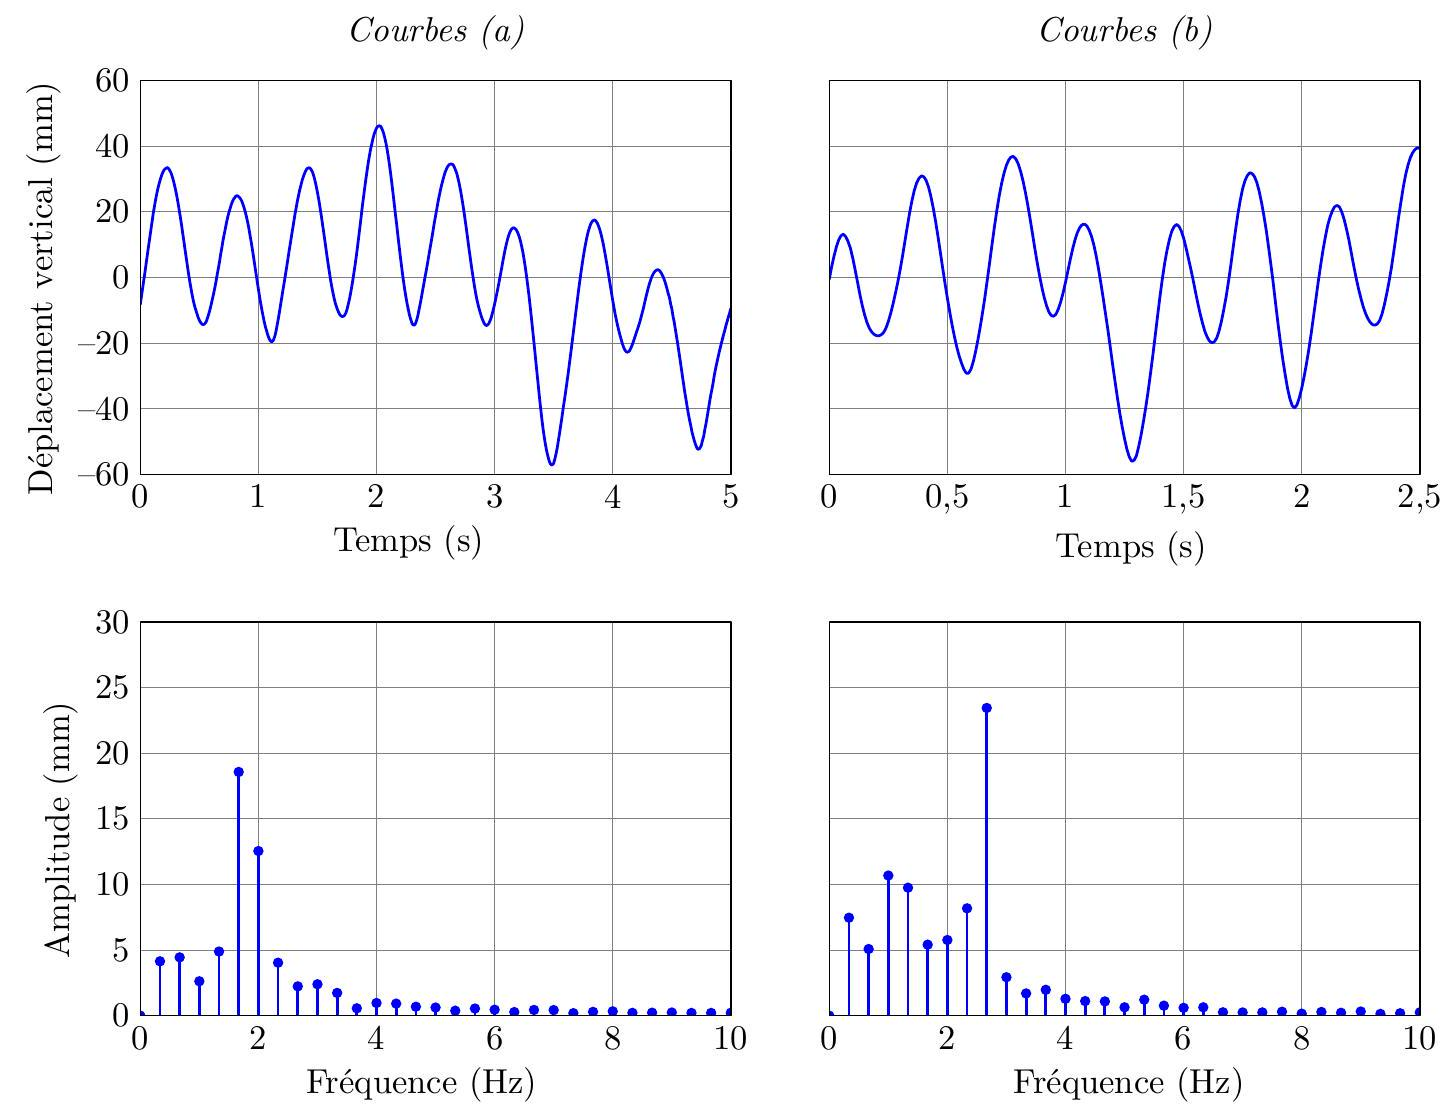
\includegraphics[width=.8\textwidth]{fig_03.jpg}
\caption{\label{fig:03} Représentations temporelle et spectrale du déplacement vertical des mains de l'utilisateur lors de la capture du mouvement}
\end{figure}
\fi
 
%Q 1
\question{\label{q:01} Associer chacune des courbes (a) ou (b) à l'enregistrement du mouvement pendant la marche ou la course de l'utilisateur. Il est conseillé d'analyser les caractéristiques de l'harmonique de plus grande amplitude.}
\ifprof
\begin{corrige}
Sur la courbe de fréquence (a), l’harmonique la plus grande se trouve à une fréquence de $\SI{1,66}{Hz}$.

Sur la courbe de fréquence (b), l’harmonique la plus grande se trouve à une fréquence de $\SI{2,66}{Hz}$.

La fréquence la plus plus basse (a) correspond à la marche. La fréquence la plus haute (b) correspond à la course.

\end{corrige}
\else
\fi

%Q 2. 
\question{\label{q:02} Proposer une méthode de filtrage pour atténuer les perturbations dues à la marche ou à la course de l'utilisateur tout en conservant les mouvements de translation verticale souhaités.}
\ifprof
\begin{corrige}

Pour filtrer les perturbations, il serait possible d'utiliser un filtre coupe-bande, atténuant les fréquences au voisinage de la fréquence de déplacement.
\end{corrige}
\else
\fi

\section{\label{part:2} Vérification du respect de l'exigence relative à la position d'équilibre}
\ifprof
\else
\begin{obj}
Vérifier du respect de l'exigence relative à la position d'équilibre.
\end{obj}
Le cahier des charges précise que le stabilisateur peut être utilisé avec des appareils photo de masse comprise entre \SI{0,350}{kg} et 1,550 kg (figure~\ref{fig:A}). L'objectif de cette partie est de vérifier que la conception est assez robuste vis-à-vis du facteur de masse de l'appareil photo pour satisfaire l'exigence 1.1 relative à la position d'équilibre du système.


\begin{figure}[H]
\centering
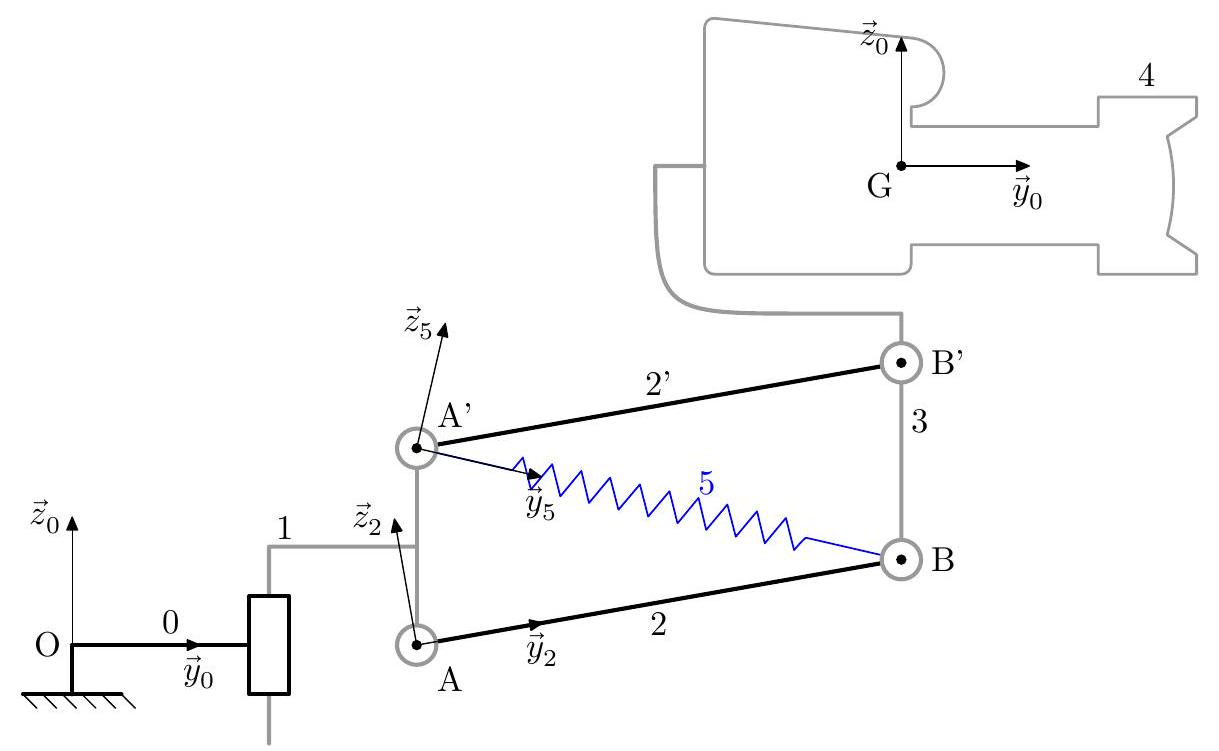
\includegraphics[width=.8\textwidth]{fig_04.jpg}
\caption{\label{fig:04} Schéma cinématique plan et paramétrage du mécanisme}
\end{figure}



Le mécanisme étudié dont la modélisation retenue est donnée (figure~\ref{fig:04}) est principalement constitué de quatre solides $\left\{(1),(2),\left(2^{\prime}\right),(3)\right\}$ formant un parallélogramme et guidés deux à deux en rotation par des liaisons modélisées par des pivots aux points A, A', B et B'. La nacelle gyrostabilisée est schématisée par la barre (3). Le support (1), faisant l'objet d'une liaison encastrement avec la perche, est supposé être en mouvement de translation par rapport au sol (0) autorisé par une glissière fictive. Ce modèle est paramétré par:

\begin{itemize}
  \item le repère terrestre $\mathcal{R}_{0}\left(\mathrm{O}, \vec{x}_{0}, \vec{y}_{0}, \vec{z}_{0}\right)$ supposé galiléen avec $\vec{z}_{0}$ vertical ascendant ;

  \item le repère $\mathcal{R}_{1}\left(\mathrm{~A}, \vec{x}_{0}, \vec{y}_{0}, \vec{z}_{0}\right)$ lié au support (1) avec $\overrightarrow{\mathrm{OA}}=y_{A} \vec{y}_{0}+z_{\text {pert }} \vec{z}_{0}$;

  \item le repère $\mathcal{R}_{2}\left(\mathrm{~A}, \vec{x}_{0}, \vec{y}_{2}, \vec{z}_{2}\right)$ lié au bras (2) avec $\alpha=\left(\vec{y}_{0}, \vec{y}_{2}\right)=\left(\vec{z}_{0}, \vec{z}_{2}\right)$;

  \item le repère $\mathcal{R}_{2}^{\prime}\left(\mathrm{A}^{\prime}, \vec{x}_{0}, \vec{y}_{2}, \vec{z}_{2}\right)$ lié au bras (2') avec $\overrightarrow{\mathrm{AA}^{\prime}}=l \vec{z}_{0}$;

  \item le repère $\mathcal{R}_{3}\left(\mathrm{~B}, \vec{x}_{0}, \vec{y}_{0}, \vec{z}_{0}\right)$ lié à la nacelle gyrostabilisée (3) et à l'appareil photo (4) liés rigidement entre eux avec $\overrightarrow{\mathrm{AB}}=L \vec{y}_{2}$. Le centre d'inertie de l'ensemble $\{(3)+(4)\}$ est noté $\mathrm{G}$, avec $\overrightarrow{\mathrm{BG}}=y_{G} \vec{y}_{0}+z_{G} \vec{z}_{0} ;$

  \item le repère $\mathcal{R}_{5}\left(\mathrm{~A}^{\prime}, \vec{x}_{0}, \vec{y}_{5}, \vec{z}_{5}\right)$ est défini tel que $\overrightarrow{\mathrm{A}^{\prime} \mathrm{B}}=L_{r} \vec{y}_{5}$ avec $\beta=\left(\vec{y}_{0}, \vec{y}_{5}\right)=\left(\vec{z}_{0}, \vec{z}_{5}\right)$.

\end{itemize}

La plage de fonctionnement du mécanisme est limitée par la géométrie des bras (2) et (2') avec $\alpha \in\left[-35^{\circ}, 45^{\circ}\right]$, $l=25 \mathrm{~mm}, L=52 \mathrm{~mm}, y_{G}=5 \mathrm{~mm}$ et $z_{G}=200 \mathrm{~mm}$.

Le ressort de traction (5) de raideur $K_{r}$ et de longueur à vide $L_{r 0}$ possède une tension initiale $F_{r 0}$ lorsque $L_{r}=L_{r 0}$. Il est relié d'une part au support (1) et d'autre part au solide (3) aux points d'ancrage respectivement A' et B.

Pour cette étude :

\begin{itemize}
  \item la nacelle gyrostabilisée (3) et l'appareil photo (4) sont considérés comme formant un seul solide ;
  \item la masse et les inerties des solides sont négligées mis à part pour l'ensemble constitué de la nacelle gyrostabilisée (3) et de l'appareil photo (4) de masse $m_{34}=m_{3}+m_{4}$ avec $m_{3}=1,250 \mathrm{~kg}$ la masse de la nacelle gyrostabilisée (3) et $m_{4}$ la masse de l'appareil photo (4). La référence retenue pour décrire la position de l'appareil photo est le centre d'inertie $\mathrm{G}$ de l'ensemble constitué de la nacelle gyrostabilisée (3) et de l'appareil photo (4) dans le repère $\mathcal{R}_{0}$.

\end{itemize}


Dans cette partie, l'étude est conduite avec les hypothèses suivantes :
\begin{itemize}
  \item les quatre liaisons pivots et la liaison glissière sont parfaites ;
  \item la modélisation est plane ;
  \item il n'y pas de perturbation $\left(z_{\text {pert }}=0\right)$.
\end{itemize}
\fi

%Q 3. 
\question{\label{q:03} Exprimer les coordonnées du centre d'inertie $\mathrm{G}$ dans le repère $\mathcal{R}_{0}$ en fonction de l'angle $\alpha$ et des paramètres géométriques du système.}
\ifprof
\begin{corrige}
Exprimons le vecteur $\vect{OG}$ dans la base $\base{x_0}{y_0}{z_0}$.

\begin{align*}
\vect{OG} &=\vect{OA}+\vect{AB}+\vect{BG} \\
&=y_A\vect{y_0}+z_{\text{pert}}\vect{z_0}+L\vect{y_2}+y_G\vect{y_0}+z_{G}\vect{z_0}\\
&=y_A\vect{y_0}+z_{\text{pert}}\vect{z_0}+L\left(\cos\alpha\vect{y_0}+\sin\alpha\vect{z_0}\right)+y_G\vect{y_0}+z_{G}\vect{z_0}\\
\end{align*}

Soit au final, 
$\vect{OG} =\left(y_A+y_G+L\cos\alpha\right)\vect{y_0}+\left(z_{\text{pert}}+z_{G}+L\sin\alpha\right)\vect{z_0}$.
\end{corrige}
\else
\fi

%Q 4. 
\question{\label{q:04} En utilisant une fermeture géométrique, donner l'expression de l'angle $\beta$ en fonction de l'angle $\alpha$ et des paramètres géométriques $L$ et $l$ du système.}
\ifprof
\begin{corrige}
Dans le triangle $AA'B$ on a $\vect{AA'}+\vect{A'B}+\vect{BA}=\vect{0}$. 
En conséquence,  $l\vect{z_0}+L_r\vect{y_5}-L\vect{y_2}=\vect{0}$.

On projette cette équation dans $\rep{0}$ et on a : 
 $l\vect{z_0}+L_r\left(\cos\beta\vect{y_0}+\sin\beta\vect{z_0}\right)-L\left(\cos\alpha\vect{y_0}+\sin\alpha\vect{z_0}\right)=\vect{0}$.
 
 On a donc les équations scalaires suivantes : 
 $\left\{
 \begin{array}{l}
L_r\cos\beta-L\cos\alpha={0}\\
 l+L_r\sin\beta-L\sin\alpha={0} \\
 \end{array}
 \right.
 $. 
 
 On cherche à exprimer $\beta$ en fonction de $\alpha$ et donc à supprimer $L_r$; donc : 
  $\left\{
 \begin{array}{l}
 L_r\sin\beta=L\sin\alpha-l \\
 L_r\cos\beta=L\cos\alpha\\
 \end{array}
 \right.
 $. 
 
 En conséquence, $\boxed{\tan\beta = \dfrac{L\sin\alpha-l}{L\cos\alpha}}$.
\end{corrige}
\else
\fi

%Q 5. 
\question{\label{q:05}Exprimer la longueur $L_{r}$ du ressort de traction (5) en fonction de l'angle $\alpha$ et des paramètres géométriques du système.}
\ifprof
\begin{corrige}
En réutilisant le système d'équation précédent, on a $L_r^2 = \left(L\sin\alpha-l\right)^2+L^2\cos^2\alpha$ soit:

$$\boxed{L_r = \sqrt{L^2+l^2-2Ll\sin\alpha}}.$$
\end{corrige}
\else
\fi

\subsection{Vérification de l'exigence relative à la plage de fonctionnement}
\ifprof
\else
L'action mécanique du ressort de traction (5) sur la nacelle gyrostabilisée (3) est modélisée par le torseur $\left\{\mathcal{F}_{5 \rightarrow 3}\right\}:$

$
\left\{\mathcal{F}_{5 \rightarrow 3}\right\}=\left\{\begin{array}{c}
F_{r} \vec{y}_{5} \\
\overrightarrow{0}
\end{array}\right\}_{\mathrm{B}} .
$
\fi

%Q 6.
\question{\label{q:06}Exprimer la composante de résultante d'action mécanique $F_{r}$ en fonction de l'angle $\alpha$, des paramètres géométriques du système et des paramètres du ressort.}
\ifprof
\begin{corrige}
On a avec la définition classique de la force de rappel du ressort de traction (en tension ici) et surtout avec $L_{r0}$ la longueur à vide du ressort on a $F_r\vect{y_5}=-K_r\left(L_r-L_{r0}\right)\vect{y_5}$. En utilisant l'expression précédente:
 
$$\boxed{F_r=-K_r\left(\sqrt{L^2+l^2-2Ll\sin\alpha}-L_{r0}\right)}$$

Avec la définition de l'effort de traction donnée par l'énoncé, on peut aussi être tenté d'écrire 

$F_r\vect{y_5}=-\left[ F_{r0} + K_r\left(L_r-L_{r0}\right)\right]\vect{y_5}$. En utilisant l'expression précédente:
 
$$\boxed{F_r=-\left[F_{r0} + K_r\left(\sqrt{L^2+l^2-2Ll\sin\alpha}-L_{r0}\right)\right]}$$
\end{corrige}
\else
\fi

%Q 7. 
\question{\label{q:07}Déterminer la direction des actions mécaniques de liaison exercées par le bras (2) sur la nacelle (3) et par le bras (2') sur la nacelle (3) \textbf{On pourra raisonner en statique)}.}
\ifprof
\begin{corrige}
Il est fait l'hypothèse que le problème est plan dans le plan $\left(0,\vect{y_0},\vect{z_0}\right)$. Les torseurs d'actions mécaniques associés aux liaisons pivot d'axe $\vect{z_0}$ sont donc des glisseurs. 

Les solides (2) et (2') sont tous soumis à deux glisseurs :
\begin{itemize}
\item d'une part, $\torseurstat{F}{1}{2}$ (pivot d'axe $\axe{A}{x_0}$) et $\torseurstat{F}{3}{2}$ (pivot d'axe $\axe{B}{x_0}$) sont des glisseurs ;
\item d'autre part, $\torseurstat{F}{1}{2'}$ (pivot d'axe $\axe{A'}{x_0}$)et $\torseurstat{F}{3}{2'}$  (pivot d'axe $\axe{B'}{x_0}$) sont des glisseurs.
\end{itemize}

D'après le PFS appliqué successivement à (2) et (2'), solides soumis à deux glisseurs, alors on a 
 $\torseurstat{F}{3}{2}+\torseurstat{F}{1}{2}=\{0\}$ et
  $\torseurstat{F}{3}{2'}+\torseurstat{F}{1}{2'}=\{0\}$. Les actions mécaniques sont de même norme, de même direction (droites $(AB)$ et $(A'B')$ soit vecteur $\vect{y_2}$).
  
De plus, $\boxed{\vect{F}_{23}=F_{23}\vect{y_2}}$ et $\boxed{\vect{F}_{2'3}=F_{2'3}\vect{y_2}}$.
\end{corrige}
\else
\fi

%Q 8. 
\question{\label{q:08}Afin de déterminer la position d'équilibre de l'ensemble $\{(3)+(4)\}$, proposer sans calcul, une démarche claire qui permette d'exprimer l'effort nécessaire du ressort de traction (5) sur la nacelle gyrostabilisée (3) \textbf{On pourra raisonner en statique)}.}
\ifprof
\begin{corrige}
\begin{center}
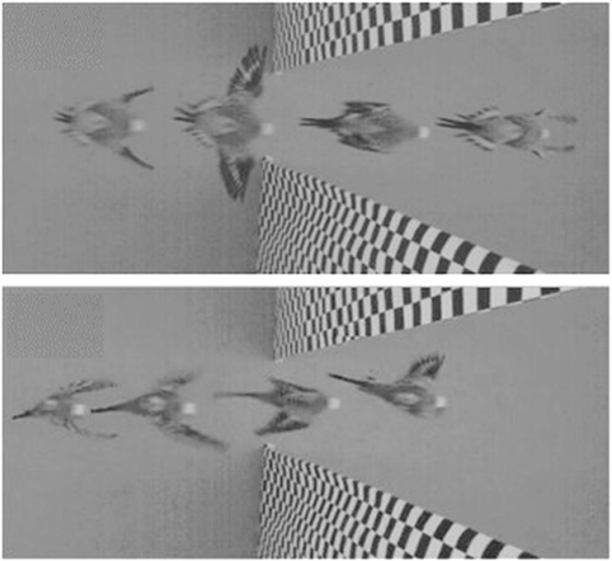
\includegraphics[width=.9\linewidth]{fig_01}
\end{center}

On isole l'ensemble \{(3)+(4)\}. 

On réalise le bilan des actions mécaniques : 
\begin{itemize}
\item action mécanique de (2') sur (3), de direction $\vect{y_2}$;
\item action mécanique de (2) sur (3), de direction $\vect{y_2}$;
\item action mécanique de la pesanteur sur \{(3)+(4)\};
\item action du ressort sur \{(3)+(4)\}.
\end{itemize}

Il faut écrire une équation du PFS permettant de ne pas faire apparaître les actions dans les deux liaisons pivot. Il faut donc réaliser un théorème de la résultante statique en projection sur $\vect{z_2}$ (perpendiculaire à $\vect{y_2}$).

\end{corrige}
\else
\fi

%Q 9. 
\question{\label{q:09}Exprimer l'équation scalaire traduisant l'équilibre du mécanisme en fonction des angles $\alpha$, $\beta$, de la masse $m_{34}$ et de la composante de résultante d'action mécanique $F_{r}$.}
\ifprof
\begin{corrige}~\\
\begin{minipage}[c]{.7\linewidth}
Calculons : 
\begin{itemize}
\item la projection de l'action du ressort sur $\vect{z_2}$ : $F_r \vect{y_5} \cdot\vect{z_2}$ $=F_r\cos\left(-\beta +\dfrac{\pi}{2}+\alpha\right)=-F_r\sin\left(\alpha-\beta \right)$;
\item la projection de l'action de pesanteur sur $\vect{z_2}$ : $-m_{34} g \vect{z_0} \cdot\vect{z_2}$ $=-m_{34} g\cos\alpha$.
\end{itemize}
On applique le TRS en projection sur $\vect{z_2}$ et on a  :
$$
\underbrace{\vectf{2'}{3}\cdot \vect{z_2}}_{\vect{0}}+\underbrace{\vectf{2}{3}\cdot \vect{z_2}}_{\vect{0}}+\vectf{\text{Pes}}{3}\cdot \vect{z_2}+\vectf{\text{Res}}{3}\cdot \vect{z_2}=0.
$$

On a donc $-m_{34} g\cos\alpha -F_r\sin\left(\alpha-\beta \right) = 0$ et  
$\boxed{F_r = -m_{34} g \dfrac{\cos\alpha}{\sin\left(\alpha-\beta \right)}}$.
\end{minipage}\hfill
\begin{minipage}[c]{.25\linewidth}
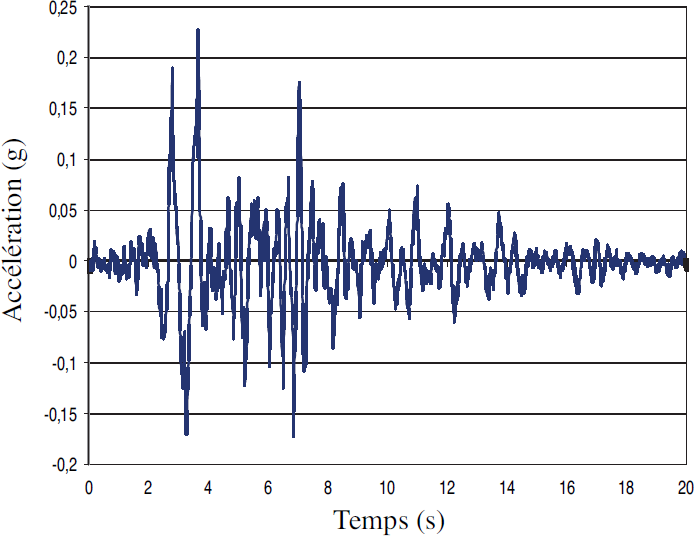
\includegraphics[width=\linewidth]{fig_02}
\end{minipage}

\end{corrige}
\else
\fi

\ifprof
\else
À partir des relations déterminées précédemment, deux fonctions \texttt{beta(alpha)} et \texttt{effort\_ressort(alpha)} qui renvoient respectivement la valeur de l'angle $\beta$ et la valeur de la composante de résultante d'action mécanique $F_{r}$ sont implantées en Python. La bibliothèque \texttt{numpy} a été importée sous le nom abrégé \texttt{np}. Les variables globales $\mathrm{g}$ et $\mathrm{m} 3$ fournissent respectivement la valeur de l'accélération de la pesanteur terrestre et la valeur de la masse de la nacelle gyrostabilisée (3). Les positions d'équilibre pour différentes valeurs de la masse $m_{4}$ sont alors obtenues par une méthode de recherche de zéro par dichotomie.
\fi

%Q 10. 
\question{\label{q:10} Écrire en Python une fonction, \texttt{fonction\_equilibre(m4, alpha)}, qui renvoie zéro lorsque, pour une valeur de masse $m_{4}$ de l'appareil photo donnée, la valeur de l'angle $\alpha$ vaut l'angle d'équilibre recherché.}
\ifprof
\begin{corrige} $\quad$
\begin{lstlisting}
def fonction_equilibre(m4,alpha):
# On donne alpha en radians
# beta(alpha) retourne un angle en radians
    return(effort_ressort(alpha)+(m3+m4)*g*(np.cos(alpha)/np.sin(alpha-beta(alpha))))
\end{lstlisting}

Cette fonction renvoie 0 si \texttt{alpha} est bien la position d'équilibre.

\end{corrige}
\else
\fi

\ifprof
\else
Une fonction \texttt{angle\_equilibre(m4)} qui renvoie la valeur de l'angle $\alpha=\alpha_{0}$ correspondant à la position d'équilibre avec une méthode de recherche de zéro par dichotomie est implantée en Python. La courbe obtenue à partir de la fonction \texttt{angle\_equilibre(m4)} représentant l'angle d'équilibre $\alpha_{0}$ en fonction de la masse de l'appareil photo $m_{4}$ est donnée (figure~\ref{fig:05}).
\fi

%Q 11. 
\question{\label{q:11} En donnant les valeurs des angles d'équilibre pour les deux valeurs extrêmes de masse, vérifier le respect de l'exigence 1.1.1. relative à la plage de fonctionnement.}
\ifprof
\begin{corrige} ~\\ $\quad$
\begin{center}
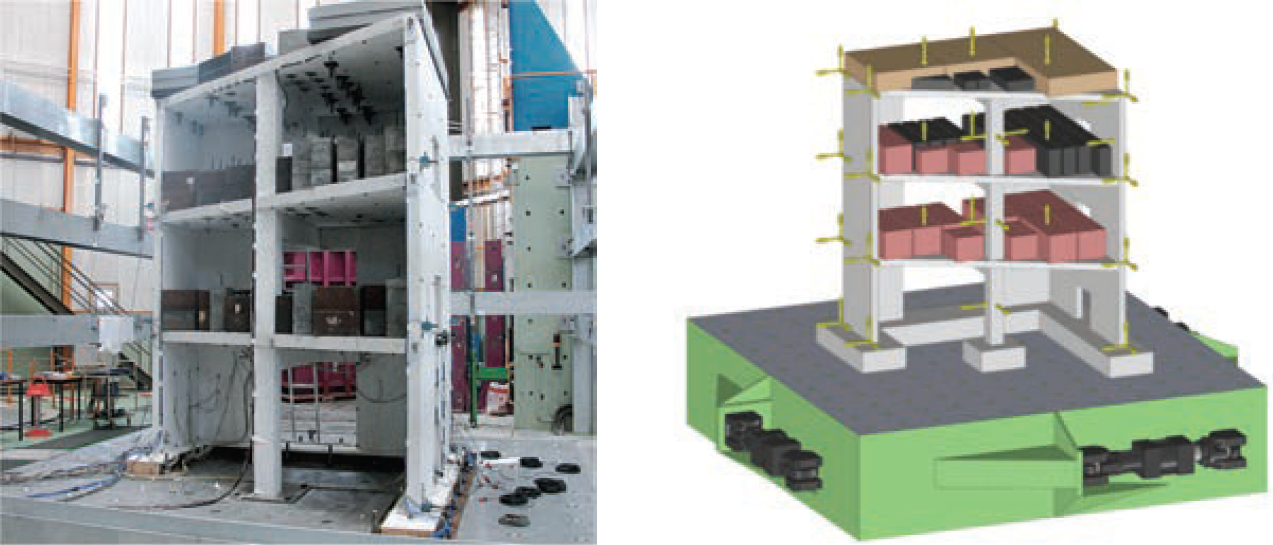
\includegraphics[width=.6\linewidth]{fig_03}
\end{center}

On peut lire en \textbf{Figure 5} que pour une masse d'appareil comprise entre 0,35 et \SI{1,55}{kg}, l'angle d'équilibre varie de $18$ à $-9\degres$. Cet intervalle est compris dans l'intervalle $\left[-35\degres,45\degres\right]$. L'exigence 1.1.1 est donc satisfaite.
\end{corrige}
\else
\fi

\subsection{Vérification de l'exigence relative au mouvement de l'appareil photo autour des positions d'équilibre possibles}
%Q 12. 
\question{\label{q:12} En étudiant le comportement du système autour des deux positions d'équilibre extrêmes, vérifier le respect de l'exigence 1.1.2. de l'appareil photo autour des positions d'équilibre possibles. Conclure sur le respect de l'exigence 1.1.}
\ifprof
\begin{corrige}
On reprend la composante verticale du vecteur $\overrightarrow{OG}$ de la \textbf{Question 3} et on regarde ses valeurs extrêmes:
\begin{itemize}
\item[$\bullet$] pour $\alpha = -9^{\circ}$: $\overrightarrow{OG}\cdot \overrightarrow{z_0} = 200 + 52\cdot \sin(-9) = \SI{191,87}{mm}$;
\item[$\bullet$] pour $\alpha = 18^{\circ}$: $\overrightarrow{OG}\cdot \overrightarrow{z_0} = 200 + 52\cdot \sin(18) = \SI{216,06}{mm}$;
\item[$\bullet$] pour $\alpha = -35^{\circ}$: $\overrightarrow{OG}\cdot \overrightarrow{z_0} = 200 + 52\cdot \sin(-35) = \SI{170,17}{mm}$;
\item[$\bullet$] pour $\alpha = 45^{\circ}$: $\overrightarrow{OG}\cdot \overrightarrow{z_0} = 200 + 52\cdot \sin(45) = \SI{236,77}{mm}$.
\end{itemize}

L'amplitude minimale autour de la position d'équilibre $\alpha = -9^{\circ}$ est alors $191,87-170,17=\SI{21,7}{mm}$, tandis qu'autour de la position  d'équilibre $\alpha = 18^{\circ}$ l'amplitude minimale est $236,77-216,06=\SI{20,71}{mm}$. Ces deux amplitudes sont bien supérieures à $\SI{20}{mm}$, ce qui satisfait l'exigence 1.1.2.\\

D'après la question précédente l'exigence 1.1.1 est satisfaite, donc l'exigence 1.1 est complètement respectée.

\end{corrige}
\else
\fi

\ifprof
\else
\begin{figure}[H]
\centering
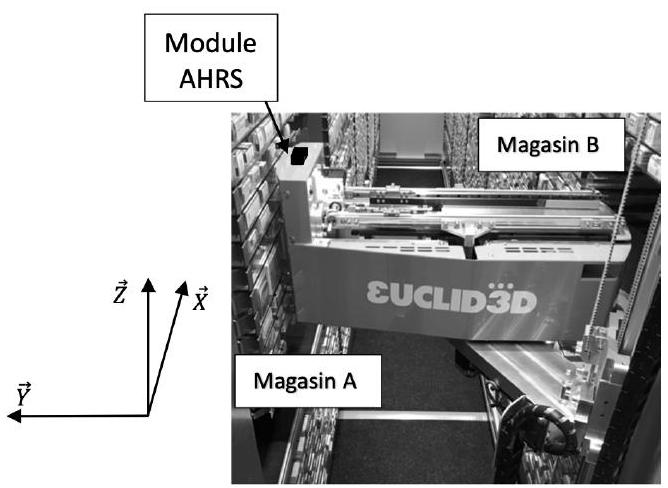
\includegraphics[width=.75\textwidth]{fig_05.jpg}
\caption{\label{fig:05} Angle d'équilibre $\alpha_{0}$ en fonction de la masse de l'appareil photo $m_{4}$}
\end{figure}
\fi


\section{\label{part:3}Détermination de la loi de mouvement du système perturbé }
\begin{obj}
Élaborer le modèle dynamique et déterminer la loi de mouvement du système perturbé afin de mettre en évidence la nécessité d'ajouter une commande active au système pour assurer le respect de l'exigence 1.2. relative à la position en mouvement du cahier des charges.
\end{obj}

\ifprof
\else
Dans cette partie, l'étude est conduite avec les hypothèses suivantes :

\begin{itemize}
  \item les quatre liaisons pivots et la liaison glissière sont parfaites ;
  \item la modélisation est plane ;
  \item le système est perturbé par l'utilisateur au niveau de la glissière (figure~\ref{fig:04}) et cette perturbation est modélisée par une fonction sinusoïdale $z_{\text {pert }}(t)=Z_{0} \sin (\omega t)$ avec l'amplitude $Z_{0}$ et la pulsation $\omega$ constantes ;
  \item à l'instant initial de cette étude, la nacelle gyrostabilisée (figure~\ref{fig:04}) est à l'équilibre.
\end{itemize}
\fi

\subsection{Détermination de la loi de mouvement}
%Q 13. 
\question{\label{q:13} En isolant l'ensemble constitué de la nacelle gyrostabilisée (3) et de l'appareil photo (4) (formant un seul solide) et en traduisant une équation scalaire issue du principe fondamental de la dynamique, donner l'équation différentielle traduisant la loi de mouvement du système. Écrire l'équation différentielle sous la forme
$
\ddot{\alpha}=C_{1} \ddot{z}_{\text {pert }} \cos \alpha+C_{2} \cos \alpha+C_{3} F_{r} \sin (\beta-\alpha)
$
en précisant l'expression des trois constantes $C_{1}, C_{2}$ et $C_{3}$ en fonction de $m_{34}, L$ et $g$.}
\ifprof
\begin{corrige}
En reprenant le raisonnement de la partie précédente, on isole \{(3)+(4)\} et on applique le TRD en projection sur $\vect{z_2}$.

Calculons $\vectrd{3}{0}=m_{34}\vectg{G}{3}{0}$ =$m_{34}\left[\dfrac{\dd \vectv{G}{3}{0}}{\dd t}\right]_{\rep{0}}$.

De plus, $\vectv{G}{3}{0}=\left[\dfrac{\dd \vect{OG}}{\dd t}\right]_{\rep{0}}$
$=\left[\dfrac{\dd \left(y_A\vect{y_0}+z_{\text{pert}}\vect{z_0}+L\vect{y_2}+y_G\vect{y_0}+z_{G}\vect{z_0}\right)}{\dd t}\right]_{\rep{0}}$

$=\left[\dfrac{\dd \left(z_{\text{pert}}\vect{z_0}+L\vect{y_2}\right)}{\dd t}\right]_{\rep{0}}$
$=\dot{z}_{\text{pert}}\vect{z_0}+L\dot{\alpha}\vect{z_2}$.

Donc, $\vectg{G}{3}{0} = \ddot{z}_{\text{pert}}\vect{z_0}+L\ddot{\alpha}\vect{z_2}-L\dot{\alpha}^2\vect{y_2}$.

Ainsi $\vectrd{3}{0}\cdot\vect{z_2} = m_{34}\ddot{z}_{\text{pert}}\cos\alpha+Lm_{34}\ddot{\alpha}$.

Le TRD en projection sur $\vect{z_2}$ donne alors 
$m_{34}\ddot{z}_{\text{pert}}\cos\alpha+Lm_{34}\ddot{\alpha} 
= -m_{34} g\cos\alpha -F_r\sin\left(\alpha-\beta \right)$.

Soit 
$$\boxed{\ddot{\alpha} 
= - \dfrac{g}{L}\cos\alpha +\dfrac{F_r}{Lm_{34}}\sin\left(\beta - \alpha \right)-\dfrac{1}{L}\ddot{z}_{\text{pert}}
\cos\alpha}$$

En identifiant, on a $C_1=-\dfrac{1}{L}$, $C_2 = -\dfrac{g}{L}$ et $C_3 = \dfrac{1}{Lm_{34}}$.
\end{corrige}
\else
\fi

\ifprof
\else
L'équation différentielle traduisant la loi de mouvement du système est du second ordre. Pour résoudre numériquement une telle équation différentielle, elle peut être réécrite sous la forme d'une équation différentielle vectorielle du premier ordre. On définit pour cela, le vecteur $A(t)$ par

$$
A(t)=\left(\begin{array}{c}
\alpha(t) \\
\dot{\alpha}(t)
\end{array}\right) .
$$

L'équation différentielle du mouvement peut alors se mettre sous la forme du problème de Cauchy

$$
\dot{A}(t)=\frac{\mathrm{d} A(t)}{\mathrm{d} t}=\left(\begin{array}{c}
\dot{\alpha}(t) \\
\ddot{\alpha}(t)
\end{array}\right)=f(A(t), t) .
$$

dont une solution peut être calculée à l'aide de la fonction \texttt{integrate.odeint} de la bibliothèque \texttt{Python} \texttt{scipy} dont le mode d'emploi est précisé dans le document réponse. 

\begin{lstlisting}
A0 =... # à  définir
t = np.arange(0,4,0.01)
A = scipy.integrate.odeint(equation_dynamique, A0, t)
\end{lstlisting}

À partir des relations déterminées précédemment, les fonctions \texttt{beta(alpha)}, \texttt{effort\_ressort(alpha)} et \texttt{angle\_equilibre(m4)} sont implantées en Python. Elles renvoient respectivement la valeur de l'angle $\beta$, la valeur de la composante de résultante d'action mécanique $F_{r}$ et la valeur de l'angle correspondant à la position d'équilibre. La bibliothèque \texttt{numpy} a été importée sous le nom abrégé \texttt{np}. Les variables globales \texttt{C1}, \texttt{C2}, \texttt{C3}, \texttt{Z0} et \texttt{w} fournissent respectivement les valeurs des trois constantes $C_{1}, C_{2}$ et $C_{3}$, de l'amplitude $Z_{0}$ et la pulsation $\omega$.
\fi

%Q 14. 
\question{\label{q:14} Écrire en Python une fonction \texttt{equation\_dynamique(A, t)} qui renvoie le vecteur dérivé $\dot{A}(t)$ en fonction du vecteur A et la date t correspondante.}
\ifprof
\begin{corrige}
On a $z_{\text{pert}}(t)=Z_0\sin\left(\omega t\right)$; 
donc $\dot{z}_{\text{pert}}(t)=Z_0\omega\cos\left(\omega t\right)$
et $\ddot{z}_{\text{pert}}(t)=-Z_0\omega^2\sin\left(\omega t\right)$
\begin{lstlisting}
def equation_dynamique(A,t):
    Ap = A[1]
    Zp = -Z0*w*w*np.sin(w*t)
    Fr = effort_ressort(A[0])
    beta = beta(alpha)
    App = C1*Zp+C2*np.cos(A[0])+C3*Fr*np.sin(beta-A[0])
    return np.array([Ap,App])
\end{lstlisting}
\end{corrige}
\else
\fi

%Q 15. 
\question{\label{q:15} Écrire l'instruction Python permettant de définir la condition initiale \texttt{A0}.}
\ifprof
\begin{corrige}
Le système est mis en oscillation librement à partir de l'instant initial. On a donc :
\begin{lstlisting}
A0 = np.array([angle_equilibre(m4),0])
\end{lstlisting}

\end{corrige}
\else
\fi

\ifprof
\else
La résolution de l'équation différentielle permet d'obtenir l'évolution de l'angle $\alpha$ au cours du temps. Le déplacement vertical de l'appareil photo est déterminé à partir de cette solution et des relations déterminées précédemment.
\fi

\subsection{Validation expérimentale du modèle dynamique}
\ifprof
\else
Pour valider le modèle dynamique, le stabilisateur vertical est soumis à une perturbation sinusoïdale $z_{\text {pert }}(t)=$ $Z_{0} \sin (\omega t)$. Les courbes expérimentales (figure~\ref{fig:06} en bas) ainsi obtenues sont à comparer avec les solutions issues de la résolution de l'équation différentielle (figure~\ref{fig:06} en haut).

\begin{figure}[H]
\centering
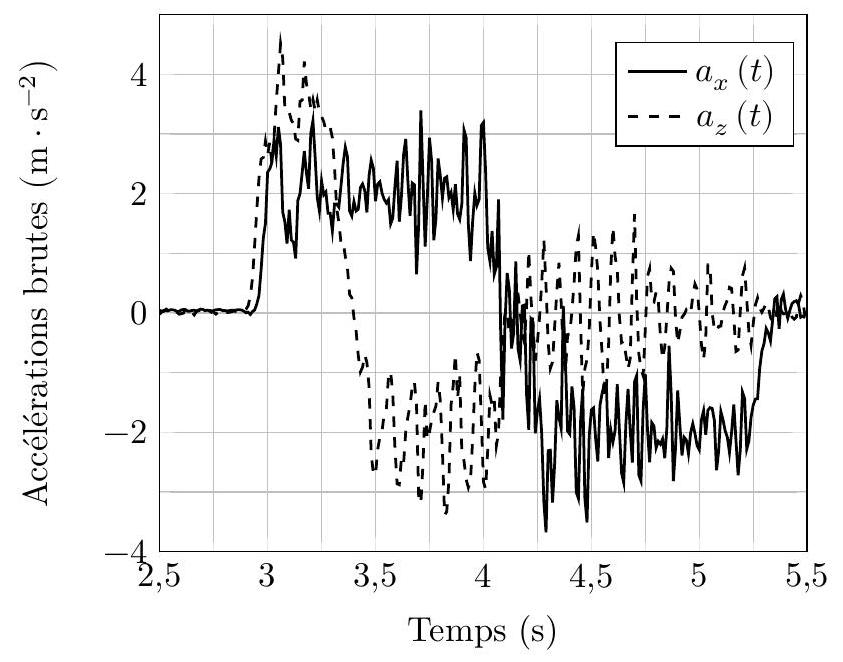
\includegraphics[width=.8\textwidth]{fig_06.jpg}
\caption{\label{fig:06} Déplacement vertical de l'appareil photo pour une perturbation d'amplitude $25 \mathrm{~mm}$ et de fréquences $1 \mathrm{~Hz}$ et $2 \mathrm{~Hz}$ avec une masse $m_{4}=1 \mathrm{~kg}$}
\end{figure}
\fi

%Q 16. 
\question{\label{q:16} Comparer les performances mesurées et simulées (figure~\ref{fig:06}). Peut-on valider le modèle dynamique pour la vérification de l'exigence 1.2. relative à la position de l'appareil photo en mouvement ? Quel phénomène physique pourrait-on prendre en compte pour améliorer le modèle ?}
\ifprof
\begin{corrige}
Pour des perturbations de fréquence de \SI{1}{Hz} ou de \SI{2}{Hz}, la fréquence et les amplitudes des signaux des réponses expérimentales et numériques sont du même ordre de grandeur. (Seule la distorsion du signal est différentes sur les 4 secondes évaluées.)

Au vu des similarités entre les signaux, le modèle dynamique doit donc pouvoir permettre de valider l'exigence~1.2 (Maîtriser la position de l’appareil photo lorsque l’utilisateur marche ou court).

Si vraiment on souhaite améliorer le modèle peut être serait-il possible d'intégrer le frottement éventuel dans les liaisons (qui contribuerait à l'amortissement du système) ou d'intégrer les masses de d'autres pièces.
\end{corrige}
\else
\fi

\subsection{Conclusion}
\ifprof
\else
Pour analyser le respect de l'exigence 1.2. relative à la position en mouvement, des simulations sont réalisées dans plusieurs configurations (figure~\ref{fig:07}).
\fi

%Q 17. 
\question{\label{q:17} Conclure sur la satisfaction de l'exigence 1.2. relative à la position de l'appareil photo en mouvement à l'aide des résultats de simulation (figure~\ref{fig:07}).}
\ifprof
\begin{corrige}
D'après l’exigence 1.2.1.1, le système doit pouvoir << Filtrer les signaux de fréquence comprise entre \SI{1,5}{Hz} et \SI{2,8}{Hz} avec une atténuation supérieure à \SI{16}{dB} et conserver les signaux
de fréquence inférieure à \SI{0,1}{Hz} avec une atténuation inférieure à \SI{3}{dB}. >>

\begin{itemize}
\item Pour une fréquence de \SI{0,1}{Hz}, le déplacement vertical mesuré est de \SI{24}{mm} soit une atténuation de $20\log \left( \dfrac{24}{25}\right) = -\SI{0,35}{dB}$. L'atténuation est donc inférieure à \SI{3}{dB}. L'exigence est validée.

\item Pour une fréquence de \SI{1,5}{Hz}, le déplacement vertical mesuré est de \SI{30}{mm} soit une atténuation de $20\log \left( \dfrac{30}{25}\right) = \SI{1,58}{dB}$. Le signal est amplifié au lieu d'être atténue. L'exigence n'est pas validée.

\item Pour une fréquence de \SI{2,8}{Hz}, le déplacement vertical mesuré est de \SI{60}{mm}. Le signal est amplifié au lieu d'être atténue. L'exigence n'est pas validée.

\end{itemize}

L'exigence~1.2 n'est donc pas satisfaite. 

\end{corrige}
\else
\fi

\ifprof
\else
Une modification des caractéristiques du ressort pourrait permettre de respecter l'exigence 1.2. relative à la position de l'appareil photo en mouvement. Néanmoins, cette modification impacterait le comportement du système à l'équilibre et ne permettrait plus de respecter l'exigence 1.1. relative à la position d'équilibre. Pour cette raison, une solution technique avec une commande active est présentée et étudiée dans la partie suivante.


\begin{figure}[H]
\centering
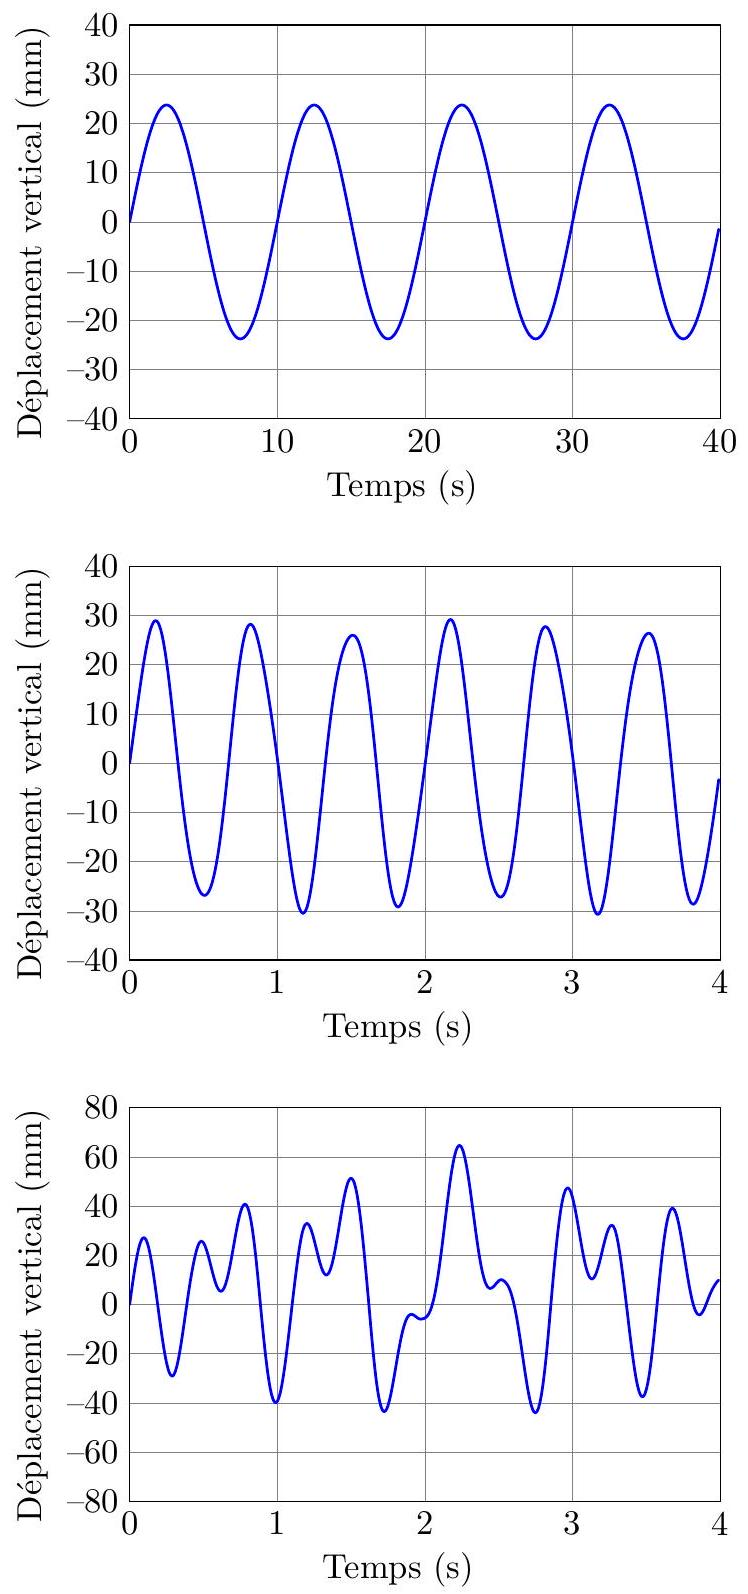
\includegraphics[width=.8\textwidth]{fig_07.jpg}
\caption{\label{fig:07} Simulations du déplacement vertical de l'appareil photo pour une perturbation d'amplitude $25 \mathrm{~mm}$ et de fréquences de $0,1 \mathrm{~Hz}, 1,5 \mathrm{~Hz}$ et $2,8 \mathrm{~Hz}$ avec des masses $m_{4}=0,350 \mathrm{~kg}$ et $m_{4}=1,550 \mathrm{~kg}$
}
\end{figure}
\fi


\section{\label{part:4} Étude d'avant-projet d'une solution technique avec une commande active }

\begin{obj}
Modéliser la commande et déterminer le réglage du correcteur. Spécifier la motorisation.
\end{obj}

\ifprof
\else
Dans cette partie, la régulation en hauteur de l'ensemble constitué de la nacelle gyrostabilisée (3) et de l'appareil photo (4) est réalisée par un motoréducteur dont le stator est lié au support (1) et dont l'arbre de sortie entraine le bras (2) (figure~\ref{fig:08}). Le rendement de la chaine de motorisation est supposé parfait.

\begin{figure}[H]
\centering
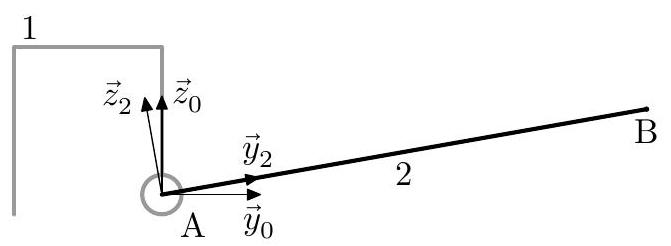
\includegraphics[width=.5\textwidth]{fig_08.jpg}
\caption{\label{fig:08} Modèle simplifié}
\end{figure}

 Les grandeurs utilisées dans cette partie sont:

\begin{itemize}
  \item $C_{m}$ le moment du couple qui modélise l'action du moteur sur l'arbre d'entrée du réducteur ;
  \item $\omega_{m}$ la vitesse de rotation de l'arbre du moteur ;
  \item $C_{s}$ le moment du couple qui modélise l'action exercée par l'arbre de sortie du réducteur sur le bras (2) ;
  \item $\omega_{s}$ la vitesse de rotation de l'arbre de sortie du réducteur sur le bras (2);
  \item $N$ le rapport de transmission du réducteur avec $N=\omega_{m} / \omega_{s}=100$;
  \item $\alpha$ l'angle formé entre le bras (2) et le support (1) défini par $\alpha=\left(\vec{y}_{0}, \vec{y}_{2}\right)=\left(\vec{z}_{0}, \vec{z}_{2}\right)$;
  \item $F_{z}$ le modèle de la composante verticale de l'effort exercé sur l'ensemble constitué de la nacelle gyrostabilisée (3) et de l'appareil photo (4) dû au couple moteur ;
  \item $F_{p}$ le modèle de l'effort de perturbation, dû au poids de l'ensemble constitué de la nacelle gyrostabilisée (3) et de l'appareil photo (4) ;
  \item $C_{m}^{*}$ la consigne en couple sur la machine à courant continu ;
  \item $m_{34}$ la masse de l'ensemble constitué de la nacelle gyrostabilisée (3) et de l'appareil photo (4) ;
  \item $L$ la longueur du bras (2).
\end{itemize}

Un diagramme des exigences partiel du stabilisateur vertical avec la commande active est donné figure~\ref{fig:B} du document réponse.

Les effets de masse et d'inertie du solide (2) sont négligeables devant les autres actions mises en jeu.
\fi

%Q 18. 
\question{\label{q:18} En retenant le schéma simplifié (figure~\ref{fig:08}) et en modélisant par un glisseur dont la résultante est notée $\vec{F}_{2 \rightarrow 3}=F_{y} \vec{y}_{0}+F_{z} \vec{z}_{0}$ l'action mécanique exercée au point B par le bras (2) sur la nacelle gyrostabilisée (3), exprimer $C_{s}$ en fonction de $F_{z}, F_{y}, \alpha(t)$ et $L$. En négligeant $F_{y}$ devant $F_{z}\left(F_{y} \approx 0\right)$ donner alors la relation entre $C_{m}, F_{z}, \alpha(t), L$ et $N$.
}



\ifprof
\begin{corrige}
On isole le bras (2), il est soumis à:
\begin{itemize}
\item[$\bullet$] l'action de (3) sur (2) au point B: $\{ \mathcal{T}_{3\to2} \} = \begin{Bmatrix} \overrightarrow{F}_{3\to2} = -\overrightarrow{F}_{2\to3} = -F_y \vec{y}_0 - F_z \vec{z}_0 \\ \overrightarrow{0} \end{Bmatrix}_B$;
\item[$\bullet$] l'action du couple en sortie de réducteur au point A: $\{ \mathcal{T}_{1\to2} \} = \begin{Bmatrix} \overrightarrow{0}  \\ C_s \vec{x}_0 \end{Bmatrix}_A$;
\item[$\bullet$] l'ensemble des actions mécaniques transmissibles par la liaison pivot en A.
\end{itemize}

Pour éviter les inconnues de liaison en A, on applique le théorème du moment statique en A projeté selon $\overrightarrow{x_0}$:

$$ C_s + (\overrightarrow{AB} \wedge \overrightarrow{F}_{3 \to 2})\cdot \overrightarrow{x_0} = 0 \quad \Rightarrow \quad C_s + L\cdot F_y\sin(\alpha) - L\cdot F_z\cos{\alpha} = 0 $$

Le rendement de la chaîne de motorisation étant parfait on a $C_m = \dfrac{1}{N}C_s$ donc en supposant $F_y \approx 0$ on obtient finalement:

$$ \boxed{C_m = \dfrac{L}{N}F_z\cos(\alpha(t))} $$
\end{corrige}
\else
\fi

\ifprof
\else
La machine à courant continu est modélisée comme un générateur de couple parfait, en particulier instantané. Le schéma-bloc de la boucle ouverte non corrigée du système est donné (figure~\ref{fig:09}) en faisant l'approximation des petits angles.

\begin{figure}[H]
\centering
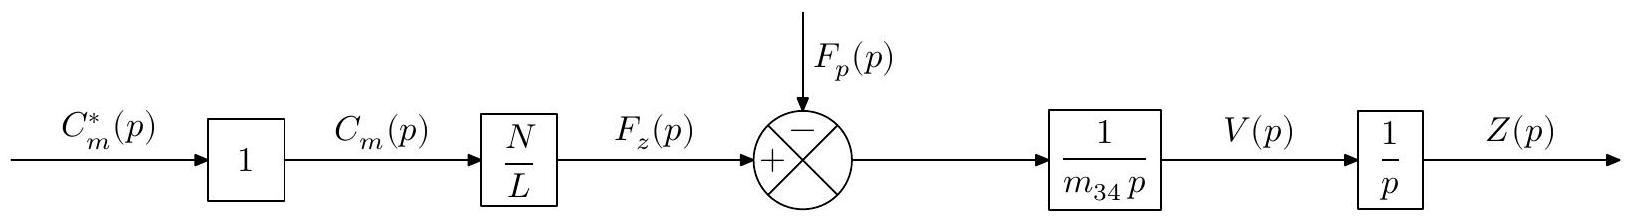
\includegraphics[width=.95\textwidth]{fig_09.jpg}
\caption{\label{fig:09} Schéma-blocs de la boucle ouverte non corrigée}
\end{figure}


Pour réaliser un asservissement, un comparateur forme la différence entre une consigne en position notée $\Delta Z^{*}(p)$ et une mesure de la hauteur $\Delta Z(p)$ de l'appareil photo renvoyée par un capteur. Cette différence est corrigée par un correcteur de fonction de transfert notée $C(p)$. En pratique, $\Delta Z(p)$ correspond à l'écart par rapport à une position de référence non présentée ici. Le capteur est modélisé par un gain unitaire. Le schéma-bloc d'asservissement est donné (figure~\ref{fig:10}).

\begin{figure}[H]
\centering
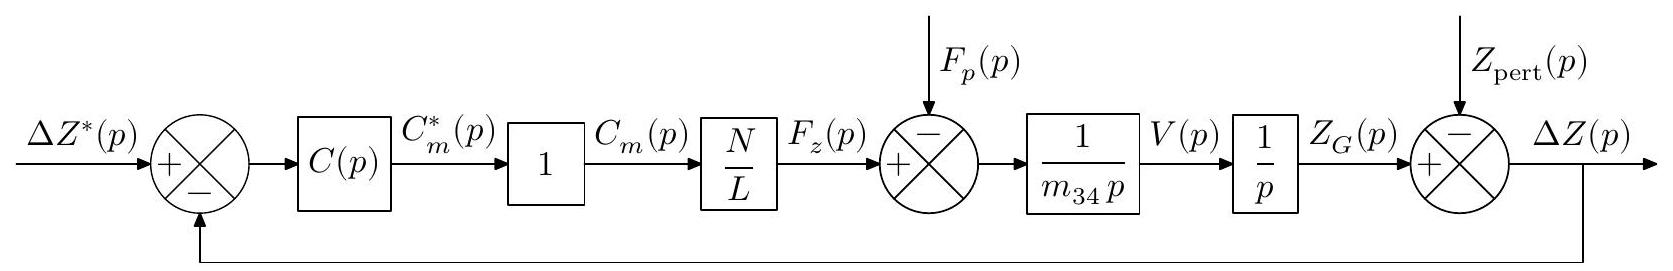
\includegraphics[width=.95\textwidth]{fig_10.jpg}
\caption{\label{fig:10} Schéma-blocs de l'asservissement de position avec un correcteur $C(p)$}
\end{figure}
\fi

\subsection{Choix et réglage du correcteur}
\ifprof
\else
Dans cette sous-partie, après avoir mis en évidence la nécessité d'introduire un correcteur, l'objet est d'en régler les paramètres de manière à ce que les performances du système vérifient les exigences du cahier des charges (figure~\ref{fig:B}).
\fi

%Q 19. 
\question{\label{q:19} Montrer qu'un correcteur proportionnel $C(p)=K$ ne permet pas d'assurer la stabilité du système en boucle fermée. On pourra raisonner sur les critères de stabilité sur la fonction de transfert en boucle ouverte ou en boucle fermée.}
\ifprof
\begin{corrige}
La fonction de transfert en poursuite s'écrit $\dfrac{\Delta Z(p)}{\Delta Z^*(p)}=\dfrac{\dfrac{KN}{Lm_{34}p^2}}{1+\dfrac{KN}{Lm_{34}p^2}}$
 $=\dfrac{KN}{Lm_{34}p^2+KN}$
  $=\dfrac{1}{\dfrac{Lm_{34}}{KN}p^2+1}$.

Plusieurs arguments permettent de répondre à la question : 
\begin{itemize}
\item il s'agit d'un système d'ordre 2 avec un coefficient d'amortissement nul; donc il s'agit d'un oscillateur harmonique non amorti. La réponse du système à un échelon est donc un sinus, ce qui n'est pas stable;
\item ce système à un pôle double à partie réelle nulle. Il est instable. 
\end{itemize}

Remarque: les fonctions de transfert en régulation ont le même dénominateur que la fonction de transfert en poursuite, l'étude de la stabilité est donc la même.

\end{corrige}
\else
\fi
\ifprof
\else

Le correcteur retenu est de la forme
$
C(p)=K\left(1+\frac{1}{T_{i} p}+T_{d} p\right) .
$

En prenant $T_{i}=2 T$ et $T_{d}=T / 2$ on obtient le correcteur sous la forme
$
C(p)=K \frac{(1+T p)^{2}}{2 T p} .
$

On pourra utiliser dans la suite la relation approximative $T_{m, \mathrm{BF}} \omega_{c, 0 \mathrm{~dB}} \approx 3$, où $T_{m, \mathrm{BF}}$ désigne le temps du premier maximum en boucle fermée et $\omega_{c, 0 \mathrm{~dB}}$ est la pulsation de coupure à $0 \mathrm{~dB}$ en boucle ouverte.

La marge de phase minimale définie dans le cahier des charges est notée $\Delta \varphi$. On se place à la limite de la valeur exigée par le cahier des charges.
\fi

%Q 20. 
\question{\label{q:20} En déduire les expressions respectives de l'argument et du module de la fonction de transfert du correcteur pour $\omega=\omega_{c, 0 \mathrm{~dB}}$ notées respectivement $\arg \left(C\left(\mathrm{j} \omega_{c, 0 \mathrm{~dB}}\right)\right)$ et $\left|C\left(\mathrm{j} \omega_{c, 0 \mathrm{~dB}}\right)\right|$ afin de vérifier l'exigence 2.3.1 relative à la stabilité de la commande active en fonction de $\omega_{c, 0 \mathrm{~dB}}, m_{34}, L, N$ et $\Delta \varphi$. On pourra raisonner sur les marges de stabilité du système.}
\ifprof
\begin{corrige}
On note $F_{\text{nc}}$  la fonction de transfert en boucle ouverte non corrigée. On a $F_{\text{nc}}(p)=\dfrac{N}{Lm_{34}p^2}$.\\

Comme on veut que le gain en boucle ouverte soit nul, on doit avoir $\left|  C(j\omega)\times \dfrac{N}{L\cdot m_{34}(j\omega)^2}\right| = 1$ donc $\boxed{\left| C\left(j\omega_{c,\SI{0}{dB}}\right)\right| = \dfrac{L\cdot m_{34}\omega_{c,\SI{0}{dB}}^2}{N}}$.\\

La phase de la boucle ouverte non corrigée $F_{nc}$ est de $-180^{\circ}$ pour tout $\omega$.\\

Le cahier des charges demande une marge de phase de 45\degres. Il faut donc que 
$\arg\left(C\left(j\omega_{c,\SI{0}{dB}}\right)\right) + \arg(F_{nc}) =-180^{\circ} + \Delta\varphi$,
soit $\boxed{\arg\left(C\left(j\omega_{c,\SI{0}{dB}}\right)\right)=\Delta\varphi}$.
\end{corrige}
\else
\fi

%Q 21. 
\question{\label{q:21} Déterminer l'expression littérale du paramètre $T$ du correcteur. Effectuer l'application numérique. (On pourra raisonner sur la marge de phase et sur le calcul de l'argument de la fonction de transfert adéquate.}
\ifprof
\begin{corrige}
$\arg\left(C\left(j\omega\right)\right)=\arg{\dfrac{K}{2T}}+2\arg\left(1+Tj\omega\right)-\arg(j\omega)=0+2\arctan\left(T\omega\right)-\dfrac{\pi}{2}$. En conséquence:
  
$\arg\left(C\left(j\omega_{c,\SI{0}{dB}}\right)\right) = 2\arctan\left(T\omega_{c,\SI{0}{dB}}\right)-\dfrac{\pi}{2}$.

Grâce à la question précédente on en déduit la relation suivante : $\boxed{T=\tan\left(\dfrac{\Delta\varphi+\dfrac{\pi}{2}}{2}\right) \dfrac{1}{\omega_{c,\SI{0}{dB}}}}$.\\
D'après le cahier des charges, on souhaite que $T_{m,\text{BF}}\leq 0,1$s. De plus, $T_{m,\text{BF}}\cdot \omega_{c,0\text{dB}} \approx 3$; on veut donc nécessairement que $\omega_{c,0\text{dB}}\approx 30$rad.s$^{-1}$.\\
Application numérique : $\boxed{T \simeq 0,08\text{s}}$.

\end{corrige}
\else
\fi

%Q 22. 
\question{\label{q:22} Déterminer l'expression littérale du paramètre $K$ du correcteur. Effectuer l'application numérique avec $m_{34}=2,8 \mathrm{~kg}, L=52 \mathrm{~mm}$ et $N=100$. (Il s'agira d'ajuster $K$ pour assurer que le gain soit nul à la pulsation calculé précédemment.)}
\ifprof
\begin{corrige}
$\left| C\left(j\omega\right)\right|= \dfrac{K}{2T}\cdot \dfrac{1+T^2\omega^2}{\omega}$. En conséquence:
$\left| C\left(j\omega_{c,\SI{0}{dB}}\right)\right| = \dfrac{K}{2T}\cdot \dfrac{1+T^2\omega_{c,\SI{0}{dB}}^2}{\omega_{c,\SI{0}{dB}}}$


On souhaite d'après la question 21 que $\left| C\left(j\omega_{c,\SI{0}{dB}}\right)\right| = \dfrac{L\cdot m_{34}\omega_{c,\SI{0}{dB}}^2}{N}$ donc  $\boxed{K=\dfrac{2TLm_{34}\omega_{c,\SI{0}{dB}}^3}{N(1+T^2\omega_{c,\SI{0}{dB}}^2)}}$.

Application numérique : $\boxed{K \simeq 0,93}$.

\end{corrige}
\else
\fi

\subsection{Spécification de l'actionneur}
\ifprof
\else
Pour concevoir le prototype, il faut définir la chaine de motorisation. Dans ce but, l'actionneur est supposé asservi. La relation entre le couple de consigne et le couple moteur est modélisé par une fonction de transfert du premier ordre

$$
\Delta(p)=\frac{C_{m}(p)}{C_{m}^{*}(p)}=\frac{1}{1+\tau p} .
$$

L'objectif de cette sous-partie est de prendre en compte le retard induit par la chaine de motorisation et les conséquences sur la stabilité. Pour spécifier au concepteur de l'actionneur la constante de temps maximale admissible $\tau$, on réalise une étude sur la stabilité en approchant au premier ordre la fonction de transfert $\Delta(p)$ par $(1-\tau p)$. La prise en compte du modèle de l'actionneur asservi se traduit par un nouveau schéma-bloc (figure~\ref{fig:11}).


\begin{figure}[H]
\centering
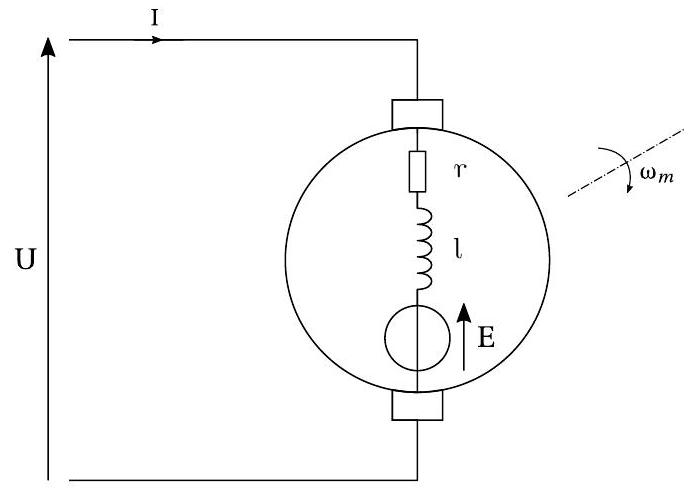
\includegraphics[width=\textwidth]{fig_11.jpg}
\caption{\label{fig:11} Schéma d'analyse de la robustesse de l'asservissement}
\end{figure}


Un critère de choix de l'actionneur sera fondé sur une étude de robustesse par rapport à la valeur maximale de ce retard acceptable pour respecter les exigences liées à la stabilité du système.

Dans cette sous-partie, l'effet de la perturbation générée par le poids sur le système n'est pas étudié.

Le système est maintenant étudié en régulation, c'est-à-dire pour lequel l'entrée notée $\Delta Z^{*}(p)=0$. Un schémabloc équivalent est donné (figure~\ref{fig:12}) en introduisant une entrée virtuelle $W(p)=0$.

\begin{figure}[H]
\centering
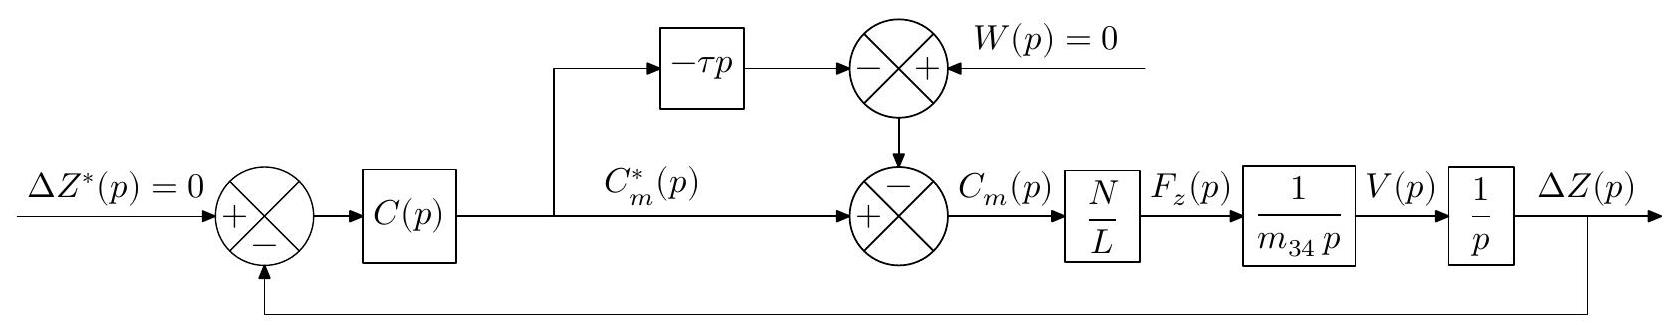
\includegraphics[width=\textwidth]{fig_12.jpg}
\caption{\label{fig:12} Schéma modifié d'analyse de la robustesse de l'asservissement}
\end{figure}
\fi


%Q 23. 
\question{\label{q:23} Donner l'expression de la fonction de transfert $H(p)$ présente dans la forme simplifiée du schéma-bloc (figure~\ref{fig:13}) en fonction de $N, L, m_{34}$ et $C(p)$.}
\ifprof
\begin{corrige}
Avec l'entrée $\Delta Z^*(p) = 0$ on peut réorganiser le schéma-bloc de la figure 12 du sujet pour le mettre sous la forme:

\begin{center}
\begin{tikzpicture}
\sbEntree{E}
\sbComp[4]{c1}{E} \sbRelier[$W(p)$]{E}{c1}
\sbCompSum[4]{c2}{c1}{+}{}{-}{} \sbRelier[]{c1}{c2}
\sbBlocL{b1}{$\dfrac{N}{Lm_{34}p^2}$}{c2}
\sbBlocL[4]{b2}{$-C(p)$}{b1} \sbRelier[$\Delta Z(p)$]{b1}{b2}
\sbSortie[4]{S}{b2}\sbRelier[$\qquad\quad C_m^*(p)$]{b2}{S}
\sbRenvoi[-3]{b2-S}{c2}{$C_m^*(p)$}

\sbDecaleNoeudy{S}{ret}
\sbBlocr[10]{r1}{$-\tau p$}{ret} \sbRelieryx{b2-S}{r1}
\sbRelierxy[]{r1}{c1}

\end{tikzpicture}
\end{center}

On exploite le signe "-" devant $C(p)$ pour modifier les signes dans le comparateur de droite:

\begin{center}
\begin{tikzpicture}
\sbEntree{E}
\sbComp[4]{c1}{E} \sbRelier[$W(p)$]{E}{c1}
\sbCompSum[4]{c2}{c1}{-}{}{+}{} \sbRelier[]{c1}{c2}
\sbBlocL{b1}{$\dfrac{N}{Lm_{34}p^2}$}{c2}
\sbBlocL[4]{b2}{$C(p)$}{b1} \sbRelier[$\Delta Z(p)$]{b1}{b2}
\sbSortie[4]{S}{b2}\sbRelier[$\qquad\quad C_m^*(p)$]{b2}{S}
\sbRenvoi[-3]{b2-S}{c2}{$C_m^*(p)$}

\sbDecaleNoeudy{S}{ret}
\sbBlocr[10]{r1}{$-\tau p$}{ret} \sbRelieryx{b2-S}{r1}
\sbRelierxy[]{r1}{c1}

\end{tikzpicture}
\end{center}

Par formule de Black on déduit $\boxed{H(p) = \dfrac{N\cdot C(p)}{L\cdot m_{34}p^2 + N\cdot C(p)}}$

\end{corrige}
\else
\fi

\ifprof
\else

\begin{figure}[H]
\centering
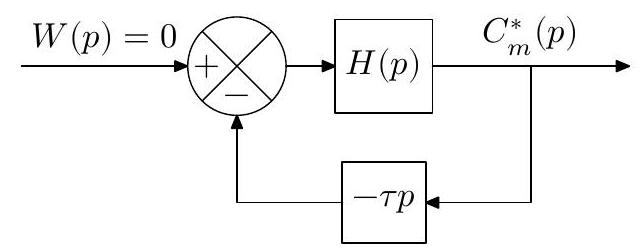
\includegraphics[width=.5\textwidth]{fig_13.jpg}
\caption{\label{fig:13} Schéma pour l'analyse de la stabilité}
\end{figure}

En pratique l'action dérivée est filtrée, l'étude du filtrage n'est pas détaillée. Les diagrammes de Bode de la fonction de transfert $H(p)$ ainsi filtrée sont donnés (figure \ref{fig:C} du document réponse). 
\fi

%Q 24. 
\question{\label{q:24} Compléter ces diagrammes sur le document réponse en représentant les diagrammes de Bode de la fonction $-\tau p$ puis tracer la fonction de transfert en boucle ouverte du système représenté en figure~\ref{fig:13} . Pour les tracés, prendre $\tau=1 \mathrm{~s}$ et faire apparaitre clairement les points de construction pour les pulsations $\omega=1 \mathrm{rad} \cdot \mathrm{s}^{-1}$, $\omega=10 \mathrm{rad} \cdot \mathrm{s}^{-1}$ et $\omega=100 \mathrm{rad} \cdot \mathrm{s}^{-1}$.}
\ifprof
\begin{corrige}
On pose $F(p) = -\tau p$. 

D'une part, 
$\arg\left(F\left(j\omega\right)\right) =\arg\left(-\tau j\omega \right)$ $=-\dfrac{\pi}{2}$.

D'autre part, 
$\left|F\left(j\omega\right)\right| =20\log\left( \tau\omega\right)$.

Pour les pulsations 
$\omega=\SI{1}{rad.s^{-1}}$, $\omega=\SI{10}{rad.s^{-1}}$ et $\omega=\SI{100}{rad.s^{-1}}$, le gain vaut donc \SI{0}{dB}, \SI{20}{dB} et \SI{40}{dB} (voir image ci-dessous).

\begin{center}
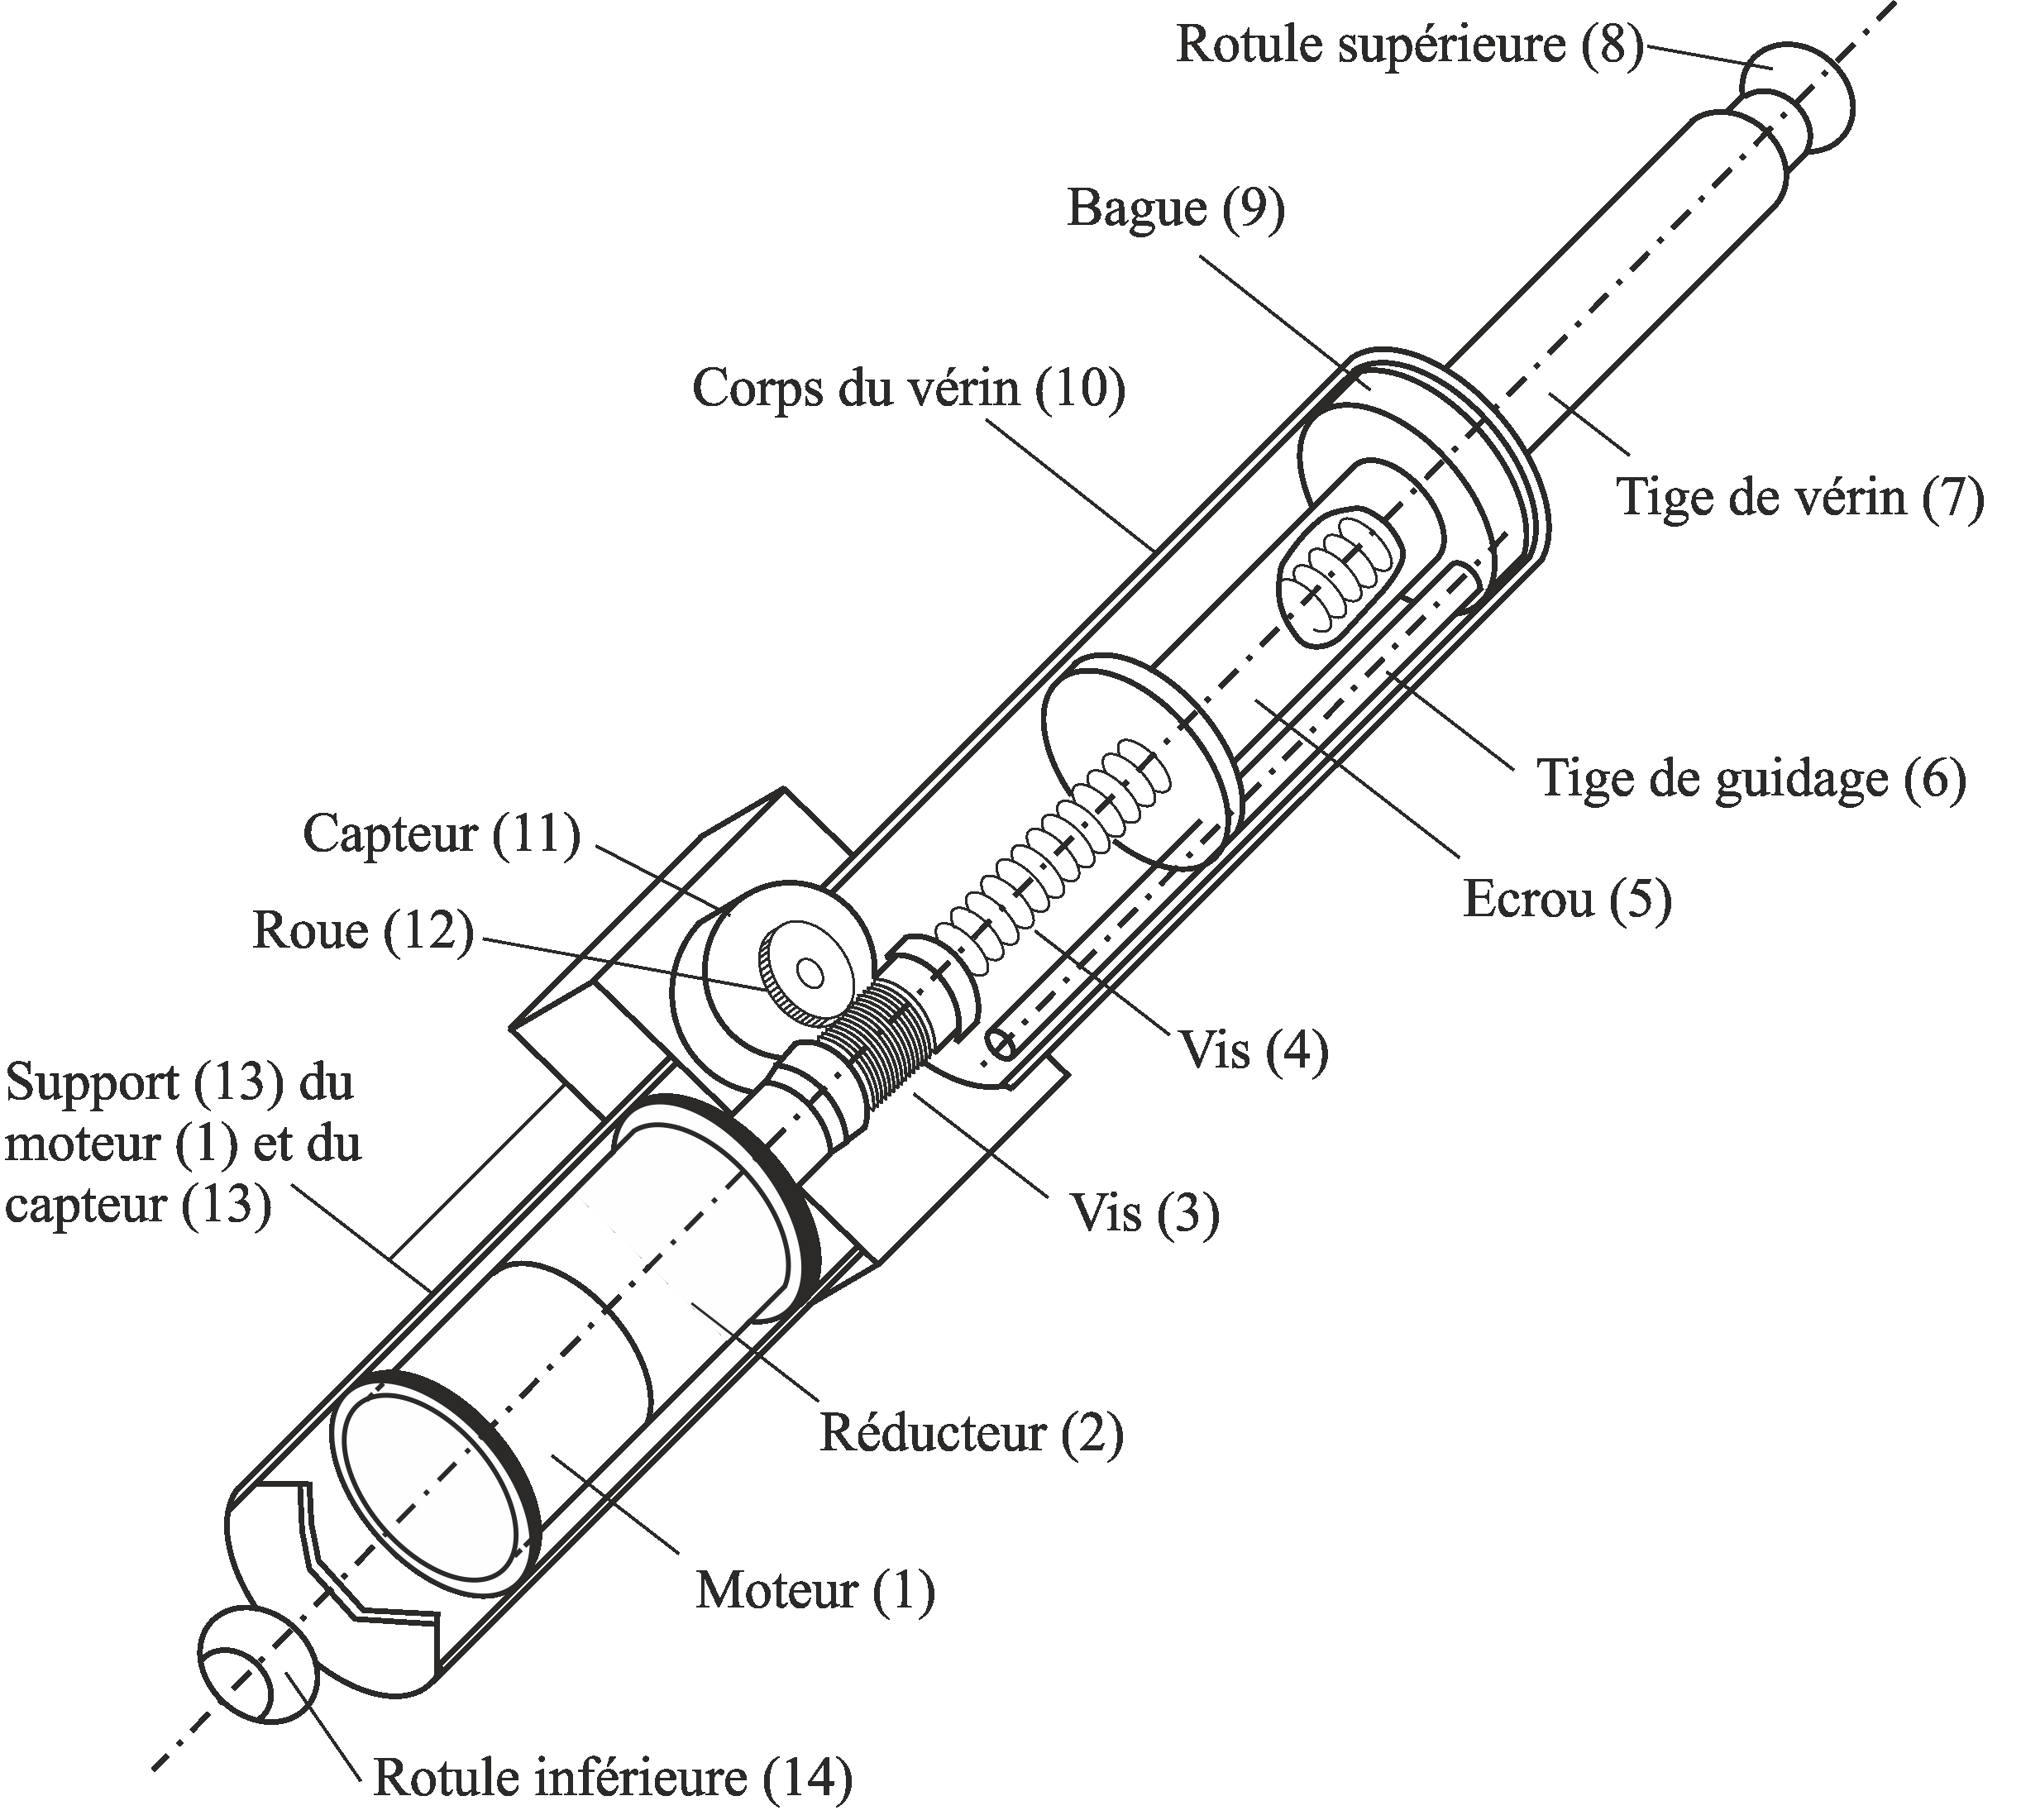
\includegraphics[width=.5\linewidth]{fig_04}
\end{center}

\end{corrige}
\else
\fi

%Q 25. 
\question{\label{q:25} En exploitant le document réponse :}
%\textit{
\begin{itemize}
  \item déterminer la valeur de $\tau$ qui assure la stabilité ;
  \item déterminer la valeur de $\tau$ qui assure un amortissement correct en considérant qu'il est obtenu lorsque la marge de phase est d'au moins $60^{\circ}$;
\item conclure sur une valeur de $\tau$ maximale admissible à spécifier pour le choix du motoréducteur.
\end{itemize}
%}
\ifprof
\begin{corrige}
On répond aux différents points dans l'ordre:
\begin{itemize}
\item Par critère du revers, le système est stable si: 
\begin{itemize}
\item le gain en dB est négatif pour une phase de -180$^{\circ}$, il faut d'après le diagramme de Bode baisser le gain de \SI{32}{dB} au minimum, soit $\tau \leq 10^{-\frac{32}{20}} = \SI{25}{ms}$;
\item la phase est supérieure à -180$^{\circ}$ lorsque le gain est nul, c'est le cas quel que soit $\tau$;
\end{itemize}
\item pour avoir une marge de phase de 60$^{\circ}$, soit obtenir une phase de $-120^{\circ}$, il faut baisser le gain d'au moins \SI{35}{dB}. On veut donc $\tau \leq 10^{-\frac{35}{20}} = \SI{18}{ms}$;
\item Par conséquent la valeur maximale de $\tau$ admissible est \textbf{\SI{18}{ms}} pour répondre au cahier des charges.
\end{itemize}

\end{corrige}
\else
\fi


\subsection{Conclusion}
\ifprof
\else
Le système est sollicité avec une consigne en échelon d'amplitude $10 \mathrm{~mm}$ à la date $t=1 \mathrm{~s}$. Le graphe représentant l'évolution de $\Delta z^{*}(t)$ et $\Delta z(t)$ est donné pour les deux valeurs extrêmes de masse de l'appareil photo (figure~\ref{fig:14}).

\begin{figure}[H]
\centering
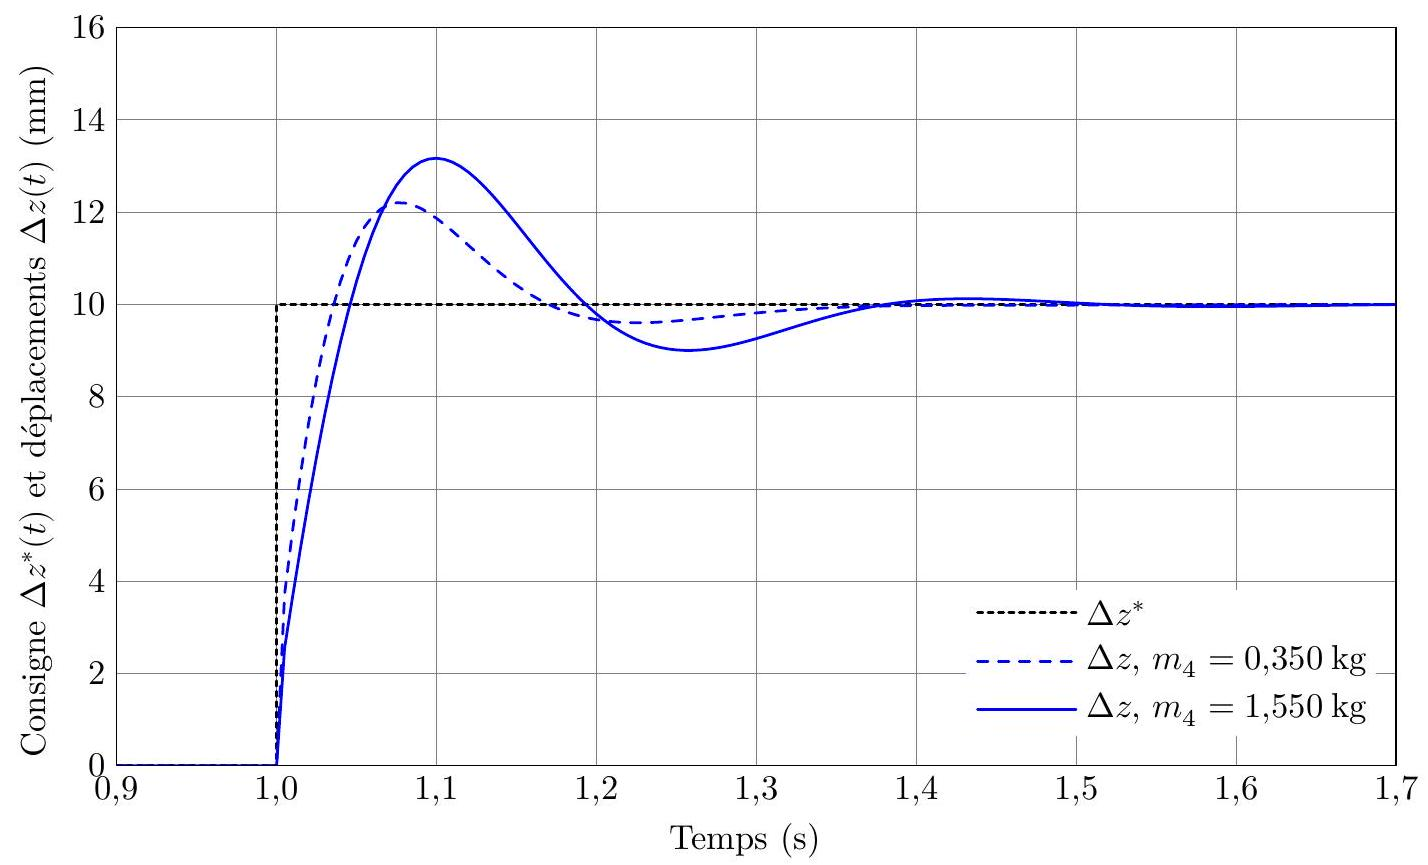
\includegraphics[width=.8\textwidth]{fig_14.jpg}
\caption{\label{fig:14}  Réponse temporelle à un échelon pour les deux valeurs extrêmes de masse de l'appareil photo}
\end{figure}
\fi

%Q 26. 
\question{\label{q:26} Conclure sur la capacité du système à satisfaire les exigences du cahier des charges (figure~\ref{fig:B}).}
\ifprof
\begin{corrige}
\begin{itemize}
\item Quelle que soit la masse de l'appareil, le premier maximum est atteint pour un temps compris entre \SI{0,05}{s} et \SI{1}{s}. L'exigence 2.1 est donc satisfaite. 
\item Quelle que soit la masse de l'appareil, l'erreur de position de l'appareil photo est nulle  en régime permanent. L'exigence 2.2 est donc satisfaite. 
\end{itemize}
Le système satisfait donc les exigences du cahier des charges. 

\end{corrige}
\else
\fi

\section{\label{part:5}Synthèse}
\begin{obj}
Analyser et comparer les deux solutions technologiques étudiées précédemment pour concevoir le stabilisateur
\end{obj}

\ifprof
\else

Une simulation numérique a été effectuée afin d'analyser la capacité des deux solutions technologiques à vérifier l'exigence 1.2.1 relative au filtrage du mouvement. Pour cela, la réponse harmonique de la fonction $Z_{G}(p) / Z_{\text {pert }}(p)$ obtenue pour le système avec commande active est comparée à celle obtenue avec le système par filtrage passif dont le modèle a été linéarisé (figure~\ref{fig:15}).

\begin{figure}[H]
\centering
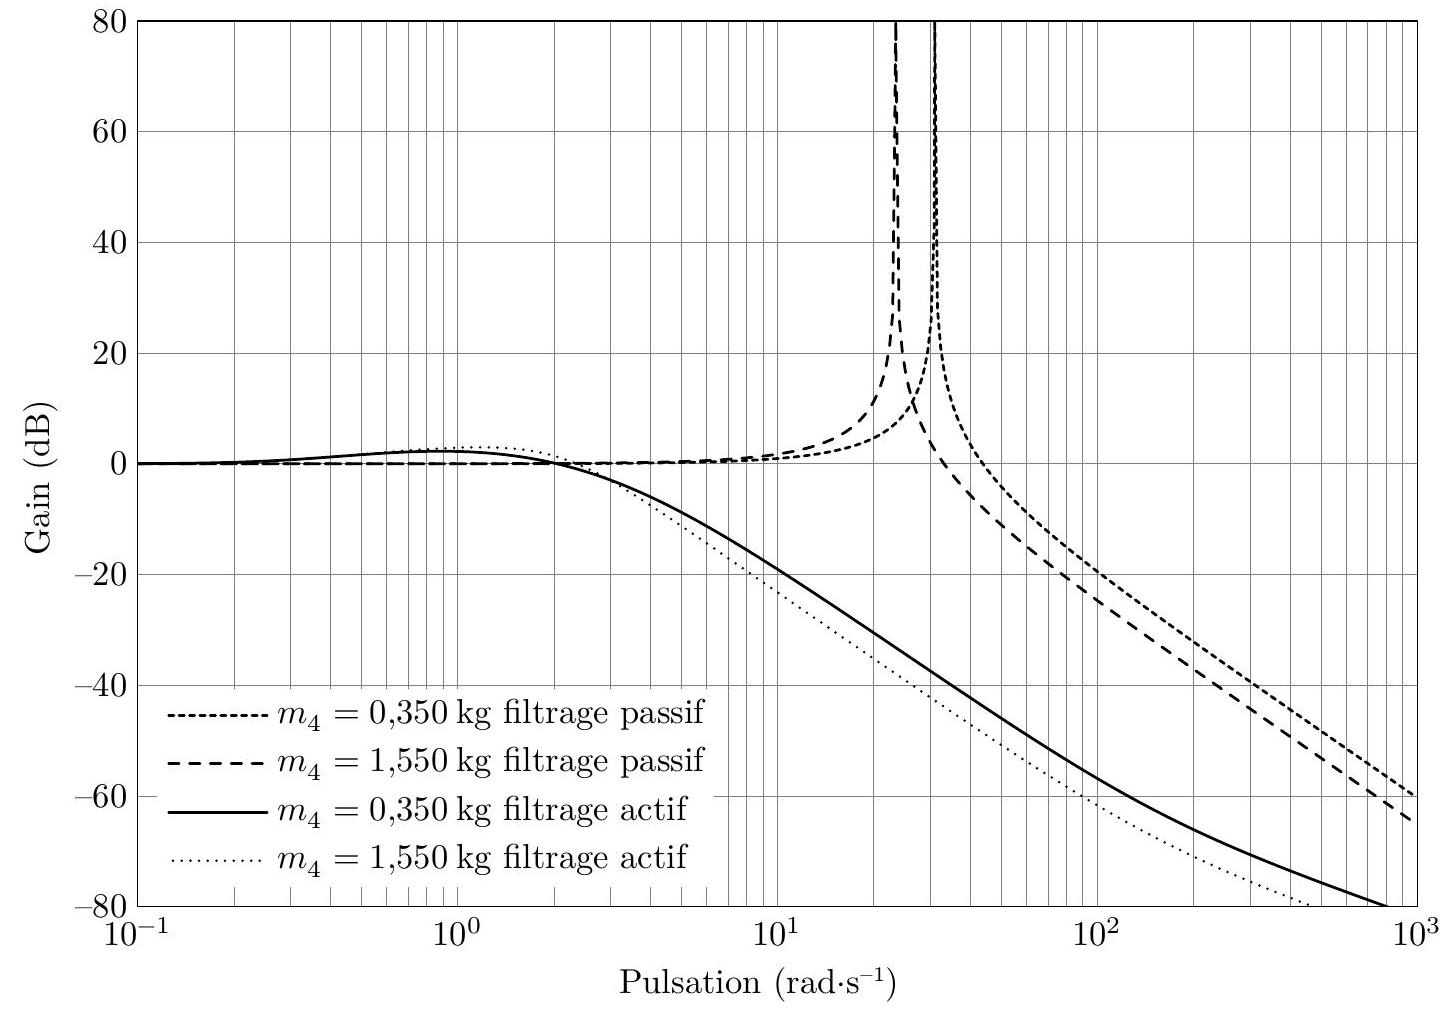
\includegraphics[width=.8\textwidth]{fig_15.jpg}
\caption{\label{fig:15}  Diagrammes de Bode de la fonction $Z_{G}(p) / Z_{\text {pert }}(p)$}
\end{figure}
\fi


%Q 27. 
\question{\label{q:27} En étudiant les réponses harmoniques (figure~\ref{fig:15}), analyser la pertinence de chacune des deux solutions technologiques étudiées à satisfaire l'exigence 1.2.1.}
\ifprof
\begin{corrige}
Entre \SI{1,5}{Hz} et \SI{2,8}{Hz}, c'est à dire entre \SI{10}{rad.s^{-1}} et \SI{20}{rad.s^{-1}} l'atténuation doit être supérieure à \SI{16}{dB}. Seul le dispositif actif permet de respecter cette exigence. 


Le dispositif passif atténue la perturbation à partir de \SI{40}{rad.s^{-1}} soient 6 pas par seconde, ce qui constitue un rythme de marche élevée.

En conclusion, il semble que le dispositif passif aura des difficultés à stabiliser l'appareil si le preneur de vu marche. En revanche, si les perturbations ont une fréquence plus haute (par exemple si le preneur de vu est sur ou dans un véhicule) le dispositif passif permettra de rejeter les perturbations. 

\end{corrige}
\else
\fi

 %Q 28. 
\question{\label{q:28}En considérant des critères de respect des performances attendues, d'encombrement, de masse, de coût et de consommation d'énergie, établir un tableau comparatif et argumenter un choix entre les deux solutions.}
\ifprof
\begin{corrige}
\begin{center}
\begin{tabular}{p{3.5cm}ccp{7cm}}
\cline{2-4}
 & Filtrage actif & Filtrage passif & Remarques \\ \hline \hline
 Performances CDC & \smiley &\frownie{}& \\ \hline
 Encombrement  &\frownie{}& \smiley&  La motorisation ajoute des composants qui peuvent nuire à l’encombrement. \\ \hline
 Masse  &\frownie{}&\smiley &La motorisation ajoute des composants qui vont augmenter la masse. \\ \hline
 Coût  &\frownie{} & \smiley& La motorisation ajoute des composants qui vont augmenter le coût. \\ \hline
 Consommation d'énergie  &\frownie{} & \smiley& La motorisation consommera davantage d'énergie qu'un système entièrement passif sans actionneur supplémentaire. \\ \hline
\end{tabular}
\end{center}

Si l'utilisateur est très exigeant sur les performances attendues du produit, il devra opter pour un filtrage actif. 


\end{corrige}
\else
\fi


\ifprof
\else
\begin{figure}[H]
\centering
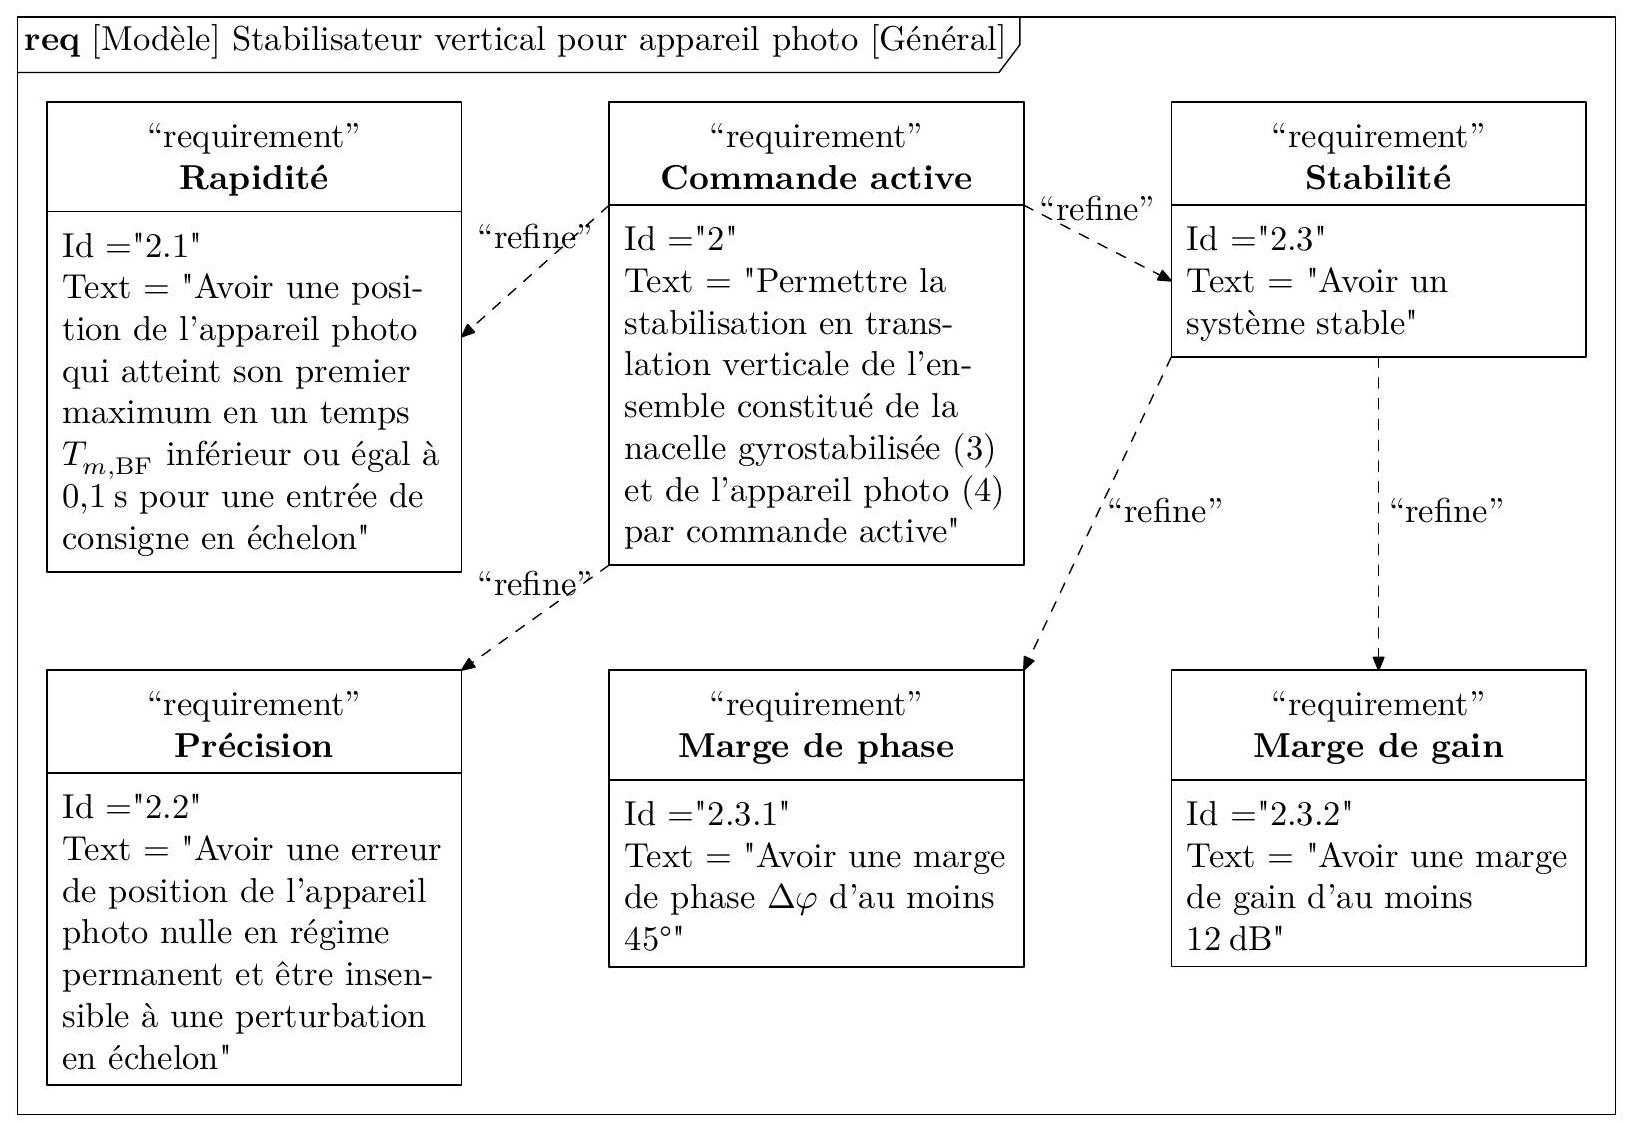
\includegraphics[width=\textwidth]{fig_16.jpg}
\caption{\label{fig:A}  Extrait du cahier des charges fonctionnel}
\end{figure}

\begin{figure}[H]
\centering
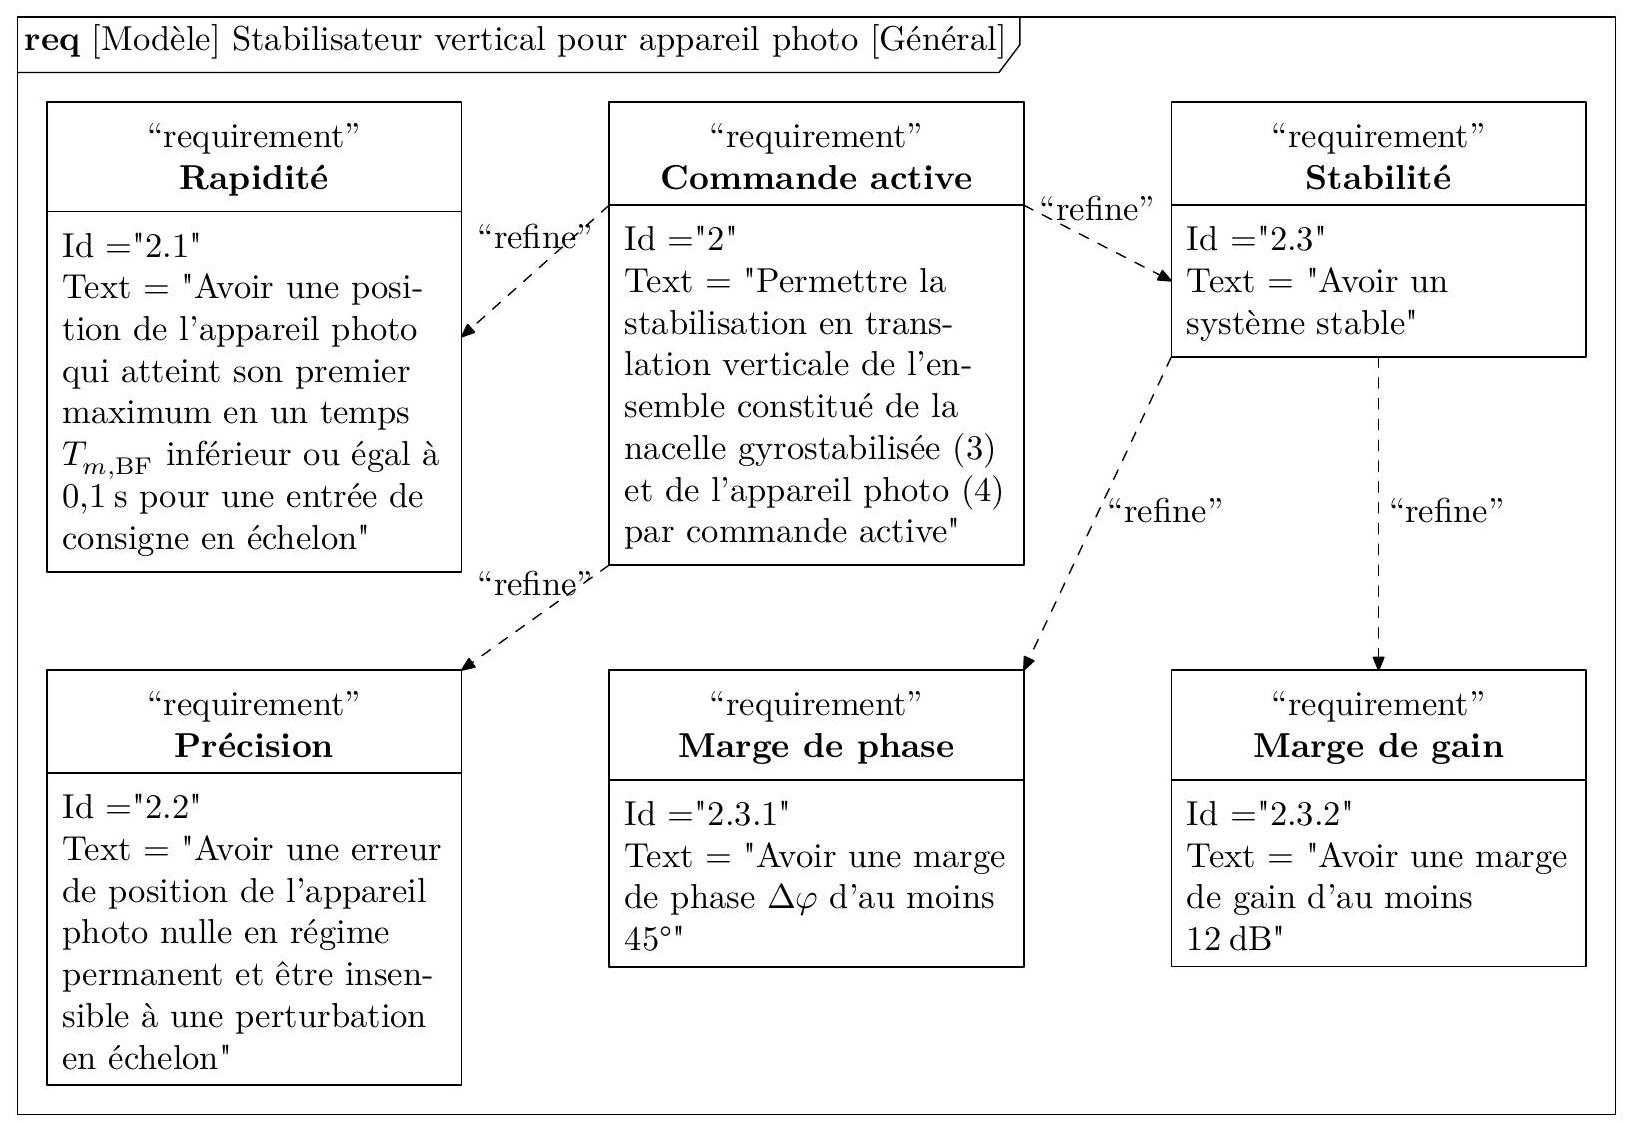
\includegraphics[width=\textwidth]{fig_17.jpg}
\caption{\label{fig:B} Diagramme des exigences partiel du stabilisateur vertical avec la commande active}
\end{figure}


\begin{figure}[H]
\centering
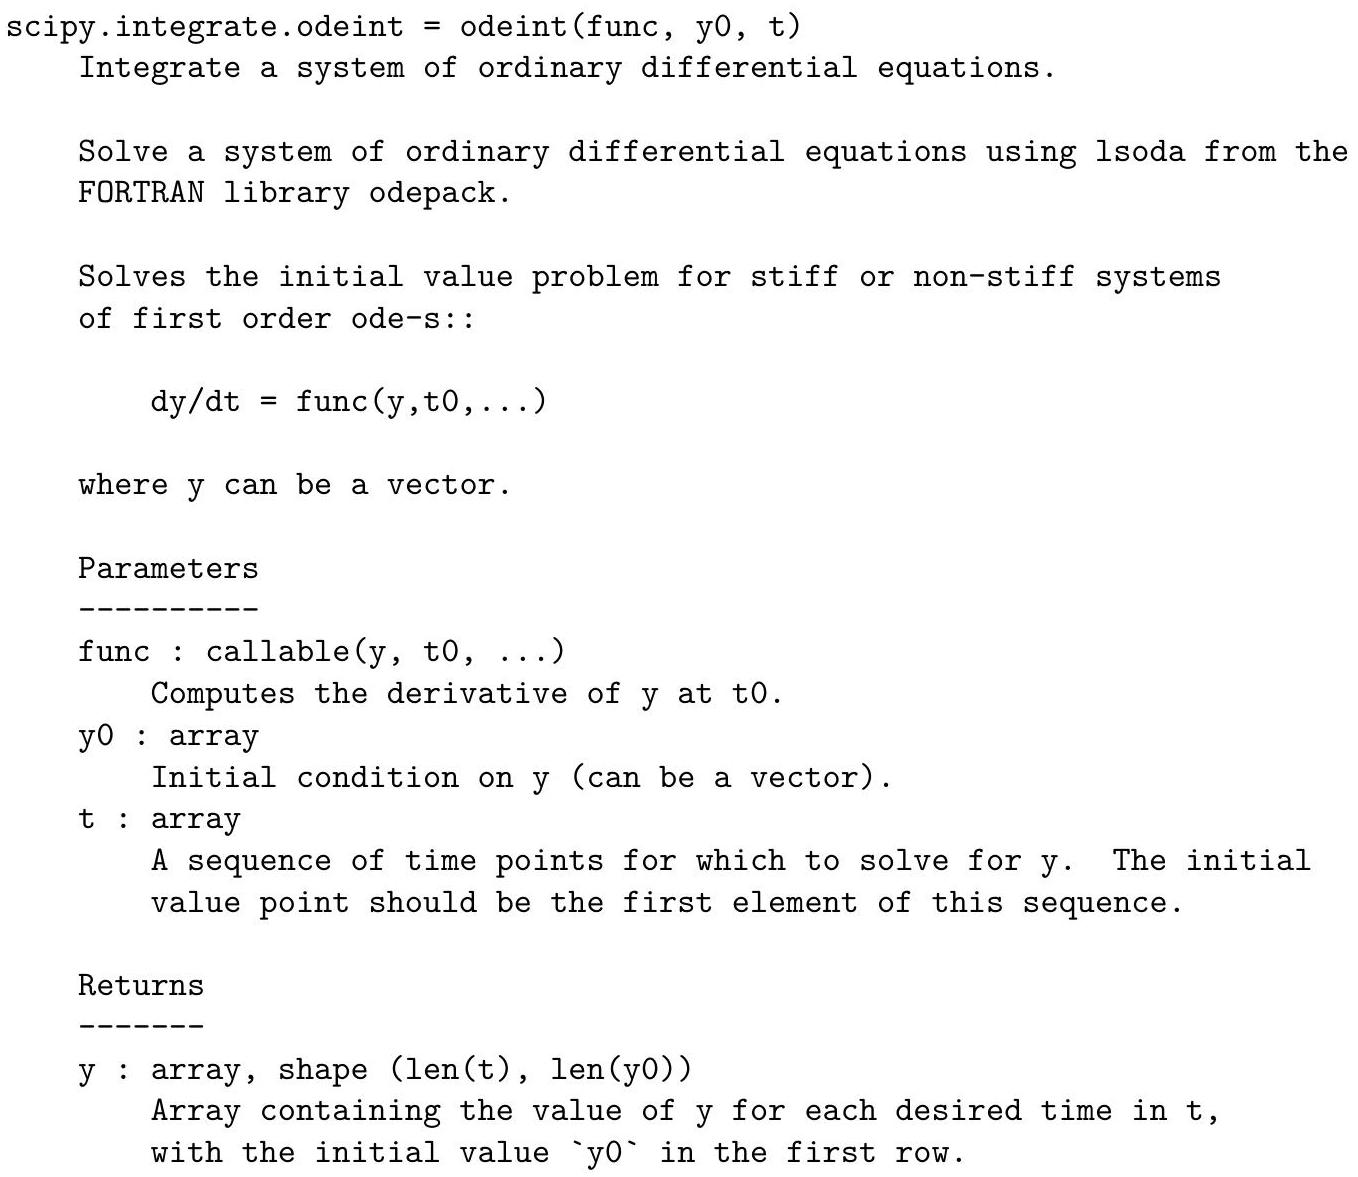
\includegraphics[width=.8\textwidth]{fig_19.jpg}
\caption{\label{fig:D} Extrait de l’aide sur la fonction Python scipy.integrate.odeint}
\end{figure}

\newpage
\section*{Document réponse}
\begin{center}
\begin{tabular}{p{0.15\textwidth}p{0.15\textwidth}|p{0.15\textwidth}p{0.15\textwidth}|p{0.15\textwidth}p{0.15\textwidth}}
\textbf{Nom : } & &
\textbf{Prénom : } &  &
\textbf{Classe : } &  \\
\hline
\end{tabular}
\end{center}

\begin{figure}[H]
\centering
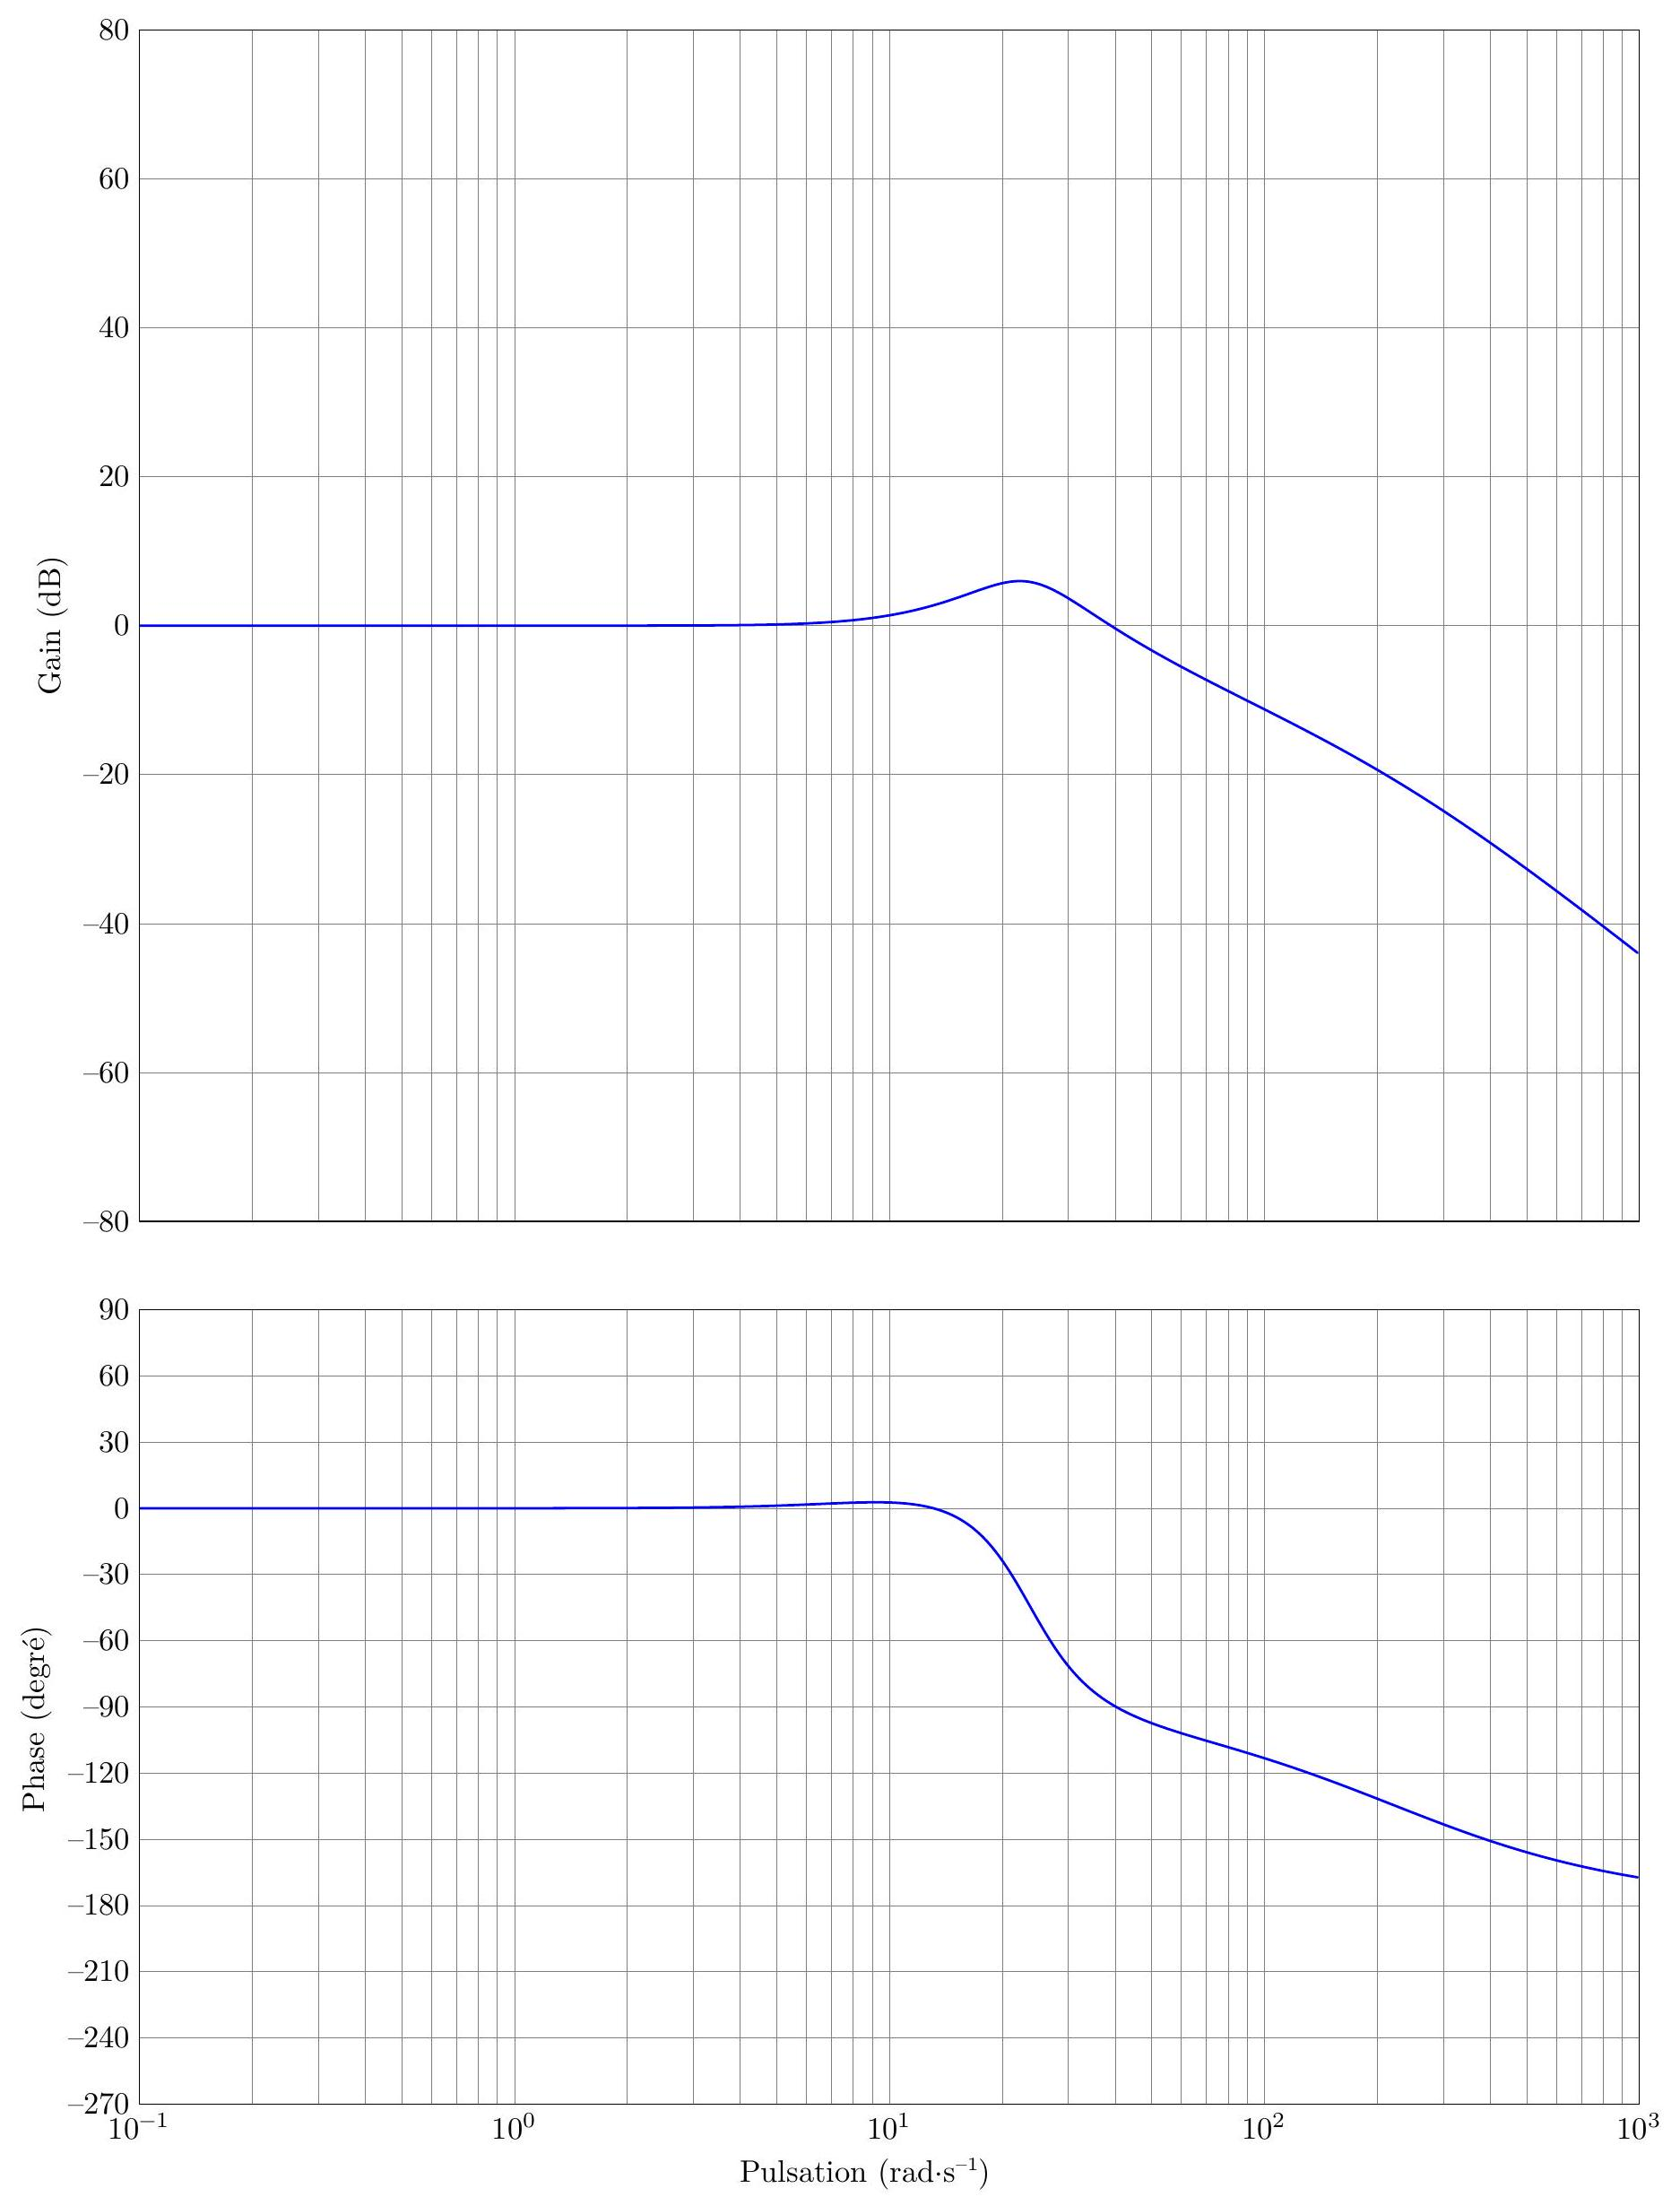
\includegraphics[width=\textwidth]{fig_18.jpg}
\caption{\label{fig:C} Diagrammes de Bode de la fonction $H(p)$ Extrait de l'aide sur la fonction Python \texttt{scipy.integrate.odeint} (Questions 24 et 25)}
\end{figure}


\fi

\newpage

\begin{tabular}{p{0.9\textwidth}}
\\
\hline
\\
\end{tabular}

\newpage

\begin{tabular}{p{0.9\textwidth}}
\\
\hline
\\
\end{tabular}

\newpage

\begin{tabular}{p{0.9\textwidth}}
\\
\hline
\\
\end{tabular}